% !TeX root = main
\documentclass[titlepage,  ngerman]{article}
\usepackage[nottoc,numbib]{tocbibind}
\usepackage[utf8]{inputenc}
\usepackage[german]{babel}
\usepackage{graphicx} 
\usepackage{amsmath, amssymb}
\usepackage[section]{placeins}
\usepackage[square,numbers]{natbib}
\bibliographystyle{abbrvnat}
\usepackage{mathtools}
\usepackage{caption}
\usepackage{subcaption}
\usepackage{chngcntr}
\counterwithin{figure}{section}
\counterwithin{equation}{section}
\counterwithin{table}{section}
\usepackage[left=3.50cm, right=3.50cm, top=3.00cm, bottom=3.00cm]{geometry}
\usepackage[normalem]{ulem}
\useunder{\uline}{\ul}{}
\usepackage{rotating}
\renewcommand{\Re}{\operatorname{\mathbb{R}e}}
\renewcommand{\Im}{\operatorname{\mathbb{I}m}}
\usepackage[hidelinks]{hyperref}
\usepackage{cleveref}

%\binoppenalty=\maxdimen
%\relpenalty=\maxdimen

\title{Aufbau und Justage eines Leckstrahlmikroskops zum Nachweis des plasmonischen Spin-Hall-Effektes}
\author{Hanno Christiansen}
\date{März 2021}

\begin{document}
	
	\maketitle
	\tableofcontents
	\newpage
	\listoffigures 
	\newpage
	
	\section{Einführung}
	Ein Leckstrahlmikroskop (engl. \textbf{L}eakage \textbf{R}adiation \textbf{M}icroscope LRM) dient der Beobachtung von Oberflächen-Plasmon-Polaritonen (engl. \textbf{S}urface \textbf{P}lasmon \textbf{P}olariton SPP). Ein SPP ist eine kollektive Ladungsdichteoszillation der freien Elektronen in einem Metall an der Grenzschicht zu einem Dielektrikum. Diese Elektronendichtewelle ist stark an das elektromagnetische Feld des Dielektrikums gebunden und eng an der Grenzschicht lokalisiert. SPP können, wenn sie an sehr dünnen Metallfilmen angeregt werden, unter bestimmten Umständen elektromagnetische Strahlung an einer zweiten Grenzschicht in ein weiteres Dielektrikum abgeben. Diese Strahlung wird als Leckstrahlung bezeichnet und kann im Fernfeld mit einem LRM beobachtet werden. Aus der Leckstrahlung können verschiedene Rückschlüsse auf die Eigenschaften des SPP gezogen werden.\cite{Drezet.2008}
	
	Da die räumliche Ausdehnung von SPP maßgeblich durch die Geometrie ihrer Trägerstruktur und nicht durch die optische Wellenlänge bestimmt wird, ist es möglich, das klassische Beugungslimit zu umgehen. Speziell können SPP auf gezielt hergestellten Strukturen genutzt werden, um auf einer Oberfläche optische Informationen zu transportieren. Außerdem reagieren SPP empfindlich auf die optischen Eigenschaften ihrer Trägerstruktur und können deswegen für Anwendungen in der Sensorik zum Einsatz kommen.\cite{Lin.2013}
	
	SPP können durch unterschiedliche Mechanismen erzeugt werden. Beispielsweise können SPP durch elektromagnetische Strahlung (EM-Strahlung) an einem Defekt auf einer Goldoberfläche angeregt werden. Der plasmonische Spin-Hall-Effekt (engl. \textbf{P}lasmonic \textbf{S}pin \textbf{H}all \textbf{E}ffect PSHE) tritt auf, wenn diese anregende EM-Strahlung elliptisch polarisiert ist und den Defekt unter streifendem Einfall trifft. Durch Nahfeldinterferenz an dem Defekt findet die SPP-Anregung dann gerichtet statt. Die effektivste Anregungsrichtung hängt hierbei von dem Drehsinn der elliptischen Polarisation ab. Dieser Effekt könnte dafür genutzt werden, die Propagationsrichtung von SPP in plasmonischen Bauteilen gezielt zu steuern. Durch die Polarisationsabhängigkeit des Effektes sind auch Anwendungen in der Sensorik denkbar.\cite{RodriguezFortuno.2013}
	
	Ziel dieser Arbeit ist es, zunächst ein vorhandenes LRM so zu modifizieren, dass eine Beobachtung des PSHE möglich wird. Im nächsten Schritt soll der PSHE dann an einem Defekt in einem Luft-Gold-Glas-System nachgewiesen werden. Im ersten Teil dieser Arbeit werden daher einige Grundlagen der Plasmonik diskutiert, die für ein Verständnis der Leckstrahlmikroskopie notwendig sind. Außerdem wird im ersten Teil auf einige Details des PSHE eingegangen. In dem Kapitel \textit{Messung und Methoden} werden das verwendete LRM und die in dieser Arbeit durchgeführten Modifikationen detailliert erläutert. Das Kapitel \textit{Ergebnisse und Diskussion} befasst sich mit der Auswertung und Interpretation der aufgezeichneten Messdaten. Abschließend werden die Ergebnisse kurz zusammengefasst, und es wird ein Ausblick auf zukünftig mögliche Projekte gegeben.
	
	\newpage	
	\section{Theorie}
	\subsection{Oberflächen-Plasmon-Polariton (SPP)}		
	Ein SPP ist das quantisierte Quasiteilchen einer an das elektromagnetische Feld gekoppelten Elektronen-Dichte-Oszillation an einer Grenzschicht zwischen einem Metall und einem Dielektrikum. Durch die spezielle Form dieser Grenzschichtgeometrie ist es möglich, trotz des rein longitudinalen Charakters der Elektronen-Dichte-Oszillation ein elektromagnetisches Feld mit transversalen Komponenten zu erzeugen. Durch die Existenz dieser transversalen Komponenten ist eine Kopplung zwischen SPP und der rein transversalen elektromagnetischen Strahlung prinzipiell möglich. Die einfachste Geometrie, in der SPP auftreten können, ist ein Zweischichtsystem. Der Halbraum oberhalb der $xy$-Ebene mit $z>0$ sei von einem Dielektrikum mit der Dielektrizitätskonstante $\epsilon_D$ ausgefüllt. Im Halbraum unterhalb der $xy$-Ebene mit $z<0$ befinde sich ein Metall mit der im allgemeinen komplexen dielektrischen Funktion $\epsilon(\omega)$ ausgefüllt. An der Grenzschicht zwischen diesen beiden Halbräumen können SPP propagieren. Um nun einige charakteristische Eigenschaften von SPP zu erläutern, wird davon ausgegangen, dass das SPP entlang der $x$-Achse propagiert und entlang der y-Achse homogen ist. So wird das Problem effektiv auf zwei Dimensionen reduziert. Wie in \cite{Maier.2007} gezeigt, lassen sich die elektromagnetischen Felder eines SPP in dieser einfachen Geometrie durch folgende Ausdrücke beschreiben:
	\begin{subequations}
		\label{eq:fields_spp}
		\begin{equation}
			\label{eq:electric_field_spp}
			\vec{E}_n(\vec{r}) = \begin{pmatrix} 1 \\ 0 \\ \pm k_{\mathrm{spp}}/k_{z,n} \end{pmatrix} E_0 \exp\left(i(k_{\mathrm{spp}}x + k_{z, n}|z|-\omega t)\right)	
		\end{equation}
		\begin{equation}
			\label{eq:magnetic_field_spp}
			\vec{H}_n\vec{r} = \begin{pmatrix} 0 \\ 1 \\ 0 \end{pmatrix} H_0 \exp\left(i(k_{\mathrm{spp}}x + k_{z, n}|z|-\omega t)\right)
		\end{equation}
	\end{subequations}
	Hierbei ist $\vec{E}_n(\vec{r})$ die elektrische Feldstärke im Material $n$ am Ort $\vec{r}$, $E_0$ die Amplitude der elektrischen Feldstärke im Ursprung, $\omega$ die Kreisfrequenz der Anregung, $x, z$ Komponenten von $\vec{r}$, $\vec{H}_n(\vec{r})$ die magnetische Feldstärke am Ort $\vec{r}$ im Medium $n$, $H_0$ die Amplitude der magnetischen Feldstärke im Ursprung und $t$ die Zeit. Der komplexe Wellenvektor der Anregung entlang der Grenzfläche ist $k_{\mathrm{spp}}$, während der senkrechte Anteil des Wellenvektors durch $k_{z,n}$ beschrieben wird.
	Der Index $n$ beschreibt hierbei das Material ($M$ für das Metall, $D$ für das Dielektrikum). 
	In dem Operator $\pm$ steht das $+$ für das Metall und das $-$ für das Dielektrikum. Der im allgemeinen komplexe Wellenvektor der Anregung $k_{\mathrm{spp}}$ ist in beiden Materialien identisch. Der Realteil $\Re\{k_{\mathrm{spp}}\}$ des komplexen Wellenvektors lässt sich in die Wellenlänge $\lambda_{\mathrm{spp}} = 2\pi/ \Re\{k_{\mathrm{spp}}\} $ des SPP umrechnen. Der Imaginärteil $\Im\{k_{\mathrm{spp}}\}$ beschreibt das Dämpfungsverhalten des SPP entlang der Ausbreitungsrichtung. Der Imaginärteil lässt sich über $L_{\mathrm{spp}} = 1/(2\Im\{k_{\mathrm{spp}}\})$ in eine Propagationslänge umrechnen.  Hierfür gilt: Nachdem das SPP eine Propagationslänge in Ausbreitungsrichtung zurückgelegt hat, sind die ursprünglichen Intensitäten des SPP auf $1/\mathrm{e}$ ihres ursprünglichen Betrages abgeklungen.
	
	Analog beschreibt $\Im\{k_{z, n}\}$ das exponentielle Abklingen der Anregung senkrecht zur Grenzfläche. Hier lassen sich die Eindringtiefen $\delta_{M,D}$ definieren. Diese drücken aus, nach welcher Entfernung senkrecht zur Grenzfläche die ursprüngliche Feldstärke auf $1/\mathrm{e}$ abgeklungen ist. Das SPP hat sowohl transversale als auch longitudinale Komponenten des elektrischen Feldes. Das magnetische Feld ist rein transversal. Daher spricht man auch von einer transversal-magnetischen Anregung (TM-Anregung).
	Der quantitative Verlauf des elektrischen Feldes ist für ein rein reelles $k_{\mathrm{spp}}$ und ein rein imaginäres $k_{z, n}$ in Abb. \ref{fig:electric_field_spp} dargestellt.
	\begin{figure}[htbp] 
		\centering
		\includegraphics[width=0.7\textwidth]{figures/E_Feld_SPP.png}
		\caption[Elektrisches Feld SPP]{Quantitativer Verlauf der EM-Felder eines SPP entlang einer Metall-Dielektrikums-Grenzschicht. Die Orientierung des elektrischen Felds ist durch die Pfeile dargestellt. Die Grauwert-Skala der Pfeile entspricht dabei dem Betrag der elektrischen Feldstärke. Die Stärke des transversalen Magnetfeldes ist durch die Farbskala dargestellt.}
		\label{fig:electric_field_spp}
	\end{figure}
	
	\subsubsection{SPP Dispersionsrelation}
	Die Herleitung der Dispersionsrelation orientiert sich an den Ausführungen in \cite[pp.~261--ff]{Fox.2020} und kann dort im Detail nachvollzogen werden. In dieser Arbeit wird sich daher nur auf eine kurze Beschreibung des Vorgehens beschränkt.
	Damit die oben angesetzten elektromagnetischen Felder \eqref{eq:fields_spp}  die Maxwell-Gleichungen \eqref{eq:maxwell} und die Randbedingungen an der Grenzschicht erfüllen, müssen die Bedingungen \eqref{eq:condition_spp_1},  \eqref{eq:condition_spp_2} gelten. (Hierbei handelt es sich um den Spezialfall nicht-magnetischer Materialien, d.h. $\mu = 1$.)
	\begin{align}
		\label{eq:maxwell}	
		&\vec{\nabla}\cdot\vec{D} = 0		&\vec{\nabla}\cdot\vec{B} = 0 \\
		&\vec{\nabla}\times\vec{E} = -\dfrac{\partial\vec{B}}{\partial t} 
		&\vec{\nabla}\times\vec{H} = 	\dfrac{\partial\vec{D}}{\partial t}\nonumber
	\end{align}
	\begin{subequations}
		\begin{equation}
			\label{eq:condition_spp_1}
			\dfrac{k_{z, M}}{\epsilon_M} + \dfrac{k_{z, D}}{\epsilon_D} = 0
		\end{equation}		
		\begin{equation}
			\label{eq:condition_spp_2}
			k_{\mathrm{spp}}^2 +k_{z, n}^2 = \epsilon_n\left(\dfrac{\omega}{c}\right)^2; \text{ für  } n=M,D
		\end{equation}
	\end{subequations}
	Hierbei ist $\vec{D}$ die dielektrische Verschiebung, $\vec{B}$ die magnetische Flussdichte, $\vec{H}$ die magnetische Feldstärke, 	$\epsilon_D$ die Permittivität des Dielektrikums und $\epsilon_M = \epsilon_M(\omega)$ die dielektrische Funktion des Metalls in Abhängigkeit von der Kreisfrequenz. Durch das Lösen der Bedingungen \eqref{eq:condition_spp_1},  \eqref{eq:condition_spp_2} ergibt sich die Dispersionsrelation des SPP an einer Grenzschicht zwischen einem Metall und einem Dielektrikum zu: 
	\begin{equation}
		\label{eq:dispersion_spp}
		\boxed{
			k_{\mathrm{spp}}\left(\omega\right) = \dfrac{\omega}{c} \sqrt{\dfrac{\epsilon_D\epsilon_M(\omega)}{\epsilon_D + 	\epsilon_M(\omega)}}  = k_0(\omega) n_{\mathrm{eff}}(\omega)}
	\end{equation}
	Hierbei ist $k_0 = \omega / c$ die Dispersion von elektromagnetischer Strahlung im Vakuum. Und $n_{\mathrm{eff}}(\omega) = \sqrt{\epsilon_D\epsilon_M(\omega)/(\epsilon_D + 	\epsilon_M(\omega))}$ wird als effektiver Brechungsindex der Anregung bezeichnet. Die Dispersion kann über den Zusammenhang $E = \hbar \omega$ auch in Abhängigkeit von der Energie dargestellt werden.
	
	Aus der Gleichung \eqref{eq:condition_spp_2} folgt $k_{z, n} = \sqrt{\epsilon_n k_0^2 - k_{\mathrm{spp}}^2}$. Diese Beziehung legt den Zusammenhang zwischen $k_{\mathrm{spp}}$ und $k_{z, n}$ fest. Außerdem lässt sich hieraus erkennen, dass für typische Materialien gilt: $ \Im\{k_{z, n}\} \gg \Re\{k_{z, n}\}$. Durch die Dominanz des Imaginärteils über den Realteil der Wellenvektorkomponente senkrecht zur Ausbreitungsrichtung fallen die Amplituden der Felder senkrecht zur Ausbreitungsrichtung exponentiell ab. Die Anregung ist daher eng an der Grenzfläche lokalisiert. 
	
	Im folgenden werden die Messdaten der dielektrischen Funktion von Gold aus der Publikation \cite{Olmon.2012} verwendet, um den Verlauf der Dispersion einer Vakuum-Gold- und einer Glas-Gold-Mode aus Gleichung \eqref{eq:dispersion_spp} zu berechnen.  Die Publikation stellt Messdaten für unterschiedliche Gold-Oberflächenrauigkeiten zur Verfügung. Es wurden die Messdaten für aufgedampftes Gold verwendet, da die in dieser Arbeit verwendeten Proben bedampft worden sind. Für die Berechnung der Dispersion der Gold-Glas-Mode wurde $\epsilon_D = 2.327$ \cite{Zeiss.} verwendet, da dies den verwendeten Proben entspricht. In der Dispersionskurve Abb. \ref{fig:dispersion_spp} ist zu erkennen, dass die Dispersionskurven bei einer Anregungs-Energie von $E = hc/\lambda_{\mathrm{HeNe}}= 1.95\,\mathrm{eV}$ jeweils rechts von der Dispersion elektromagnetischer Strahlung liegen. Es tritt bei gegebener Energie also eine Wellenvektor-Differenz zwischen SPPs und elektromagnetischer Strahlung auf. Diese $k$-Differenz sorgt dafür, dass SPPs nicht ohne weiteres von elektromagnetischer Strahlung angeregt werden können.
	\begin{figure}[h]		
		\centering
		\includegraphics[width=0.7\textwidth]{figures/dispersion.png}
		\caption[Dispersion SPP]{Dispersionskurve der Gold-Vakuum- und der Gold-Glas-Mode. Die Lichtlinien im jeweiligen Medium sind zur Orientierung gestrichelt dargestellt}
		\label{fig:dispersion_spp}		
	\end{figure}
	Die Differenz zwischen Dispersionskurve und Lichtlinie sorgt dafür, dass SPP nicht ohne weiteres von elektromagnetischer Strahlung im jeweiligen Medium angeregt werden können.	
	\subsubsection{Anregung von SPPs mittels EM-Strahlung}
	\label{sec:exictation}
	Um trotz der Wellenvektordifferenz in den Dispersionsrelationen SPPs mit elektromagnetischer Strahlung anregen zu können, ist es notwendig, den Wellenvektor der EM-Strahlung anzupassen. Hierfür gibt es unterschiedliche Mechanismen:
	\paragraph{Kretschmann-Konfiguration}
	In der Kretschmann-Konfiguration wird ausgenutzt, dass für die Anregung von SPPs mit EM-Strahlung nur die Wellenvektorkomponente parallel zur Grenzschichtebene relevant ist. Wie in Abbildung \ref{fig:dispersion_spp} dargestellt, hat EM-Strahlung im Vakuum bei gleicher Energie einen kleineren Wellenvektor als ein SPP. 
	
	In der Kretschmann-Konfiguration wird ein System aus drei Schichten verwendet (Abbildung \ref{fig:kretschman}). Ein dünner Metallfilm wird zwischen zwei Dielektrika mit $\epsilon_{D_1} > \epsilon_{D_2}$ eingeschlossen. Das SPP soll hierbei an der Grenzschicht Metall Dielektrikum 2 propagieren. In der der ersten Schicht wird der Wellenvektor der anregenden EM-Strahlung zunächst auf $k_\mathrm{D} = k_0 \sqrt{\epsilon_D}$ vergrößert. Die Permittivität des Dielektrikum 1 $\epsilon_{D_1}$ wird dabei so gewählt, dass $k_\mathrm{D_1} = k_0 \sqrt{\epsilon_{D_1}} > k_\mathrm{SPP}$ gilt. Der Einfallswinkel $\theta_E$ der EM-Strahlung auf die Grenzschichtebene wird dann so festgelegt, dass der auf die Grenzschichtebene projizierte Anteil des Wellenvektors $k_{\mathrm{D_1}\parallel} = k_{\mathrm{D_1}} \sin(\theta_E)$ exakt gleich dem Wellenvektor des SPP $k_\mathrm{SPP}$ an der Grenzschichtebene Metall-Dielektrikum 2 ist. Aus dieser Gleichheit ergibt sich die folgende Phasenanpassungsbedingung: 
	\begin{align}
		\label{eq:phase_condition_kretschmann}
		\sin(\theta_E) &= \dfrac{\Re\{k_{\mathrm{spp}}\}}{k_{D_1}}\\
		\Rightarrow \Re\{k_{\mathrm{SPP}}\} &= \sin(\theta_E) k_0 \sqrt{\epsilon_{D_1}}
	\end{align}  
	\begin{figure}[h] 
		\centering
		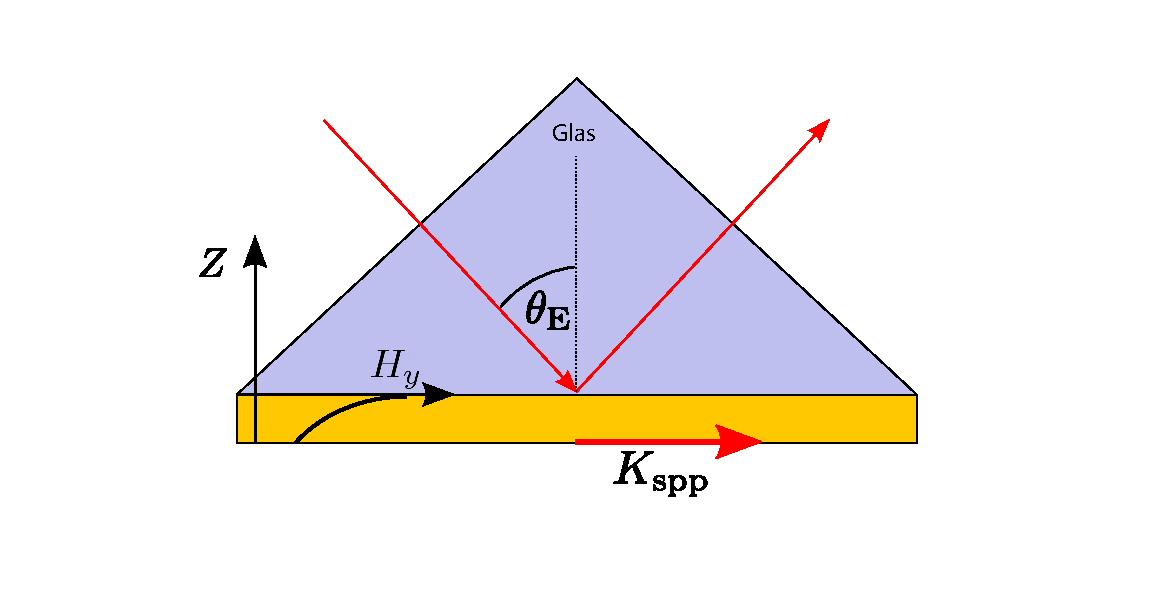
\includegraphics[width=0.5\textwidth]{figures/Kretschmann.pdf}
		\caption[Kretschmann-Konfiguration]{Schematischer Aufbau der Kretschmann-Konfiguration. Die Anregungsstrahlung tritt hier zunächst in das Medium mit $\epsilon_{D_1}$ ein. Hierdurch wird der Wellenvektor der Anregungsstrahlung auf $k_{D_1}=k_0\sqrt{\epsilon_{D_1}}$ vergrößert. Das das Dielektrikum 1 wird so gewählt, dass $k_{D_1}> k_{\mathrm{SPP}}$ gilt. ($k_{\mathrm{SPP}}$ bezieht sich hierbei auf die Mode Metall-Dielektrikum 2 und ergibt sich aus \eqref{eq:dispersion_spp}). Der Einfallswinkel $\theta_E$ wird so gewählt, dass die Projektion von $k_{D_1}$ auf die Goldoberfläche exakt $k_{\mathrm{SPP}}$ entspricht. Die Abbildung ist an \cite{Jaruschewski.2020} angelehnt.}
		\label{fig:kretschman}
	\end{figure}
	Bei der Reflexion einer elektromagnetischen Welle an einem Metall dringen in das Metall evaneszente Felder ein \cite{Novotny.2012b}. Ist die Metallschicht ausreichend dünn, haben diese evaneszenten Felder an der Grenzfläche Metall-Dielektrikum 2 noch genügend Feldstärke, um dort ein SPP anzuregen. Dies ist nur möglich, da die Wellenvektorkomponente parallel zur Grenzschichtebene wie oben erläutert, an das SPP angepasst worden sind. Die in Abb. \ref{fig:kretschman} gezeigte Geometrie nutzt für das Dielektrikum 1 einen Halbkreis, damit der Strahl unabhängig vom Winkel $\theta_\mathrm{E}$ senkrecht in das Dielektrikum 1 eintritt. Als Dielektrikum 2 wird häufig Vakuum oder Luft verwendet.			
	
	\paragraph{Anregung an Strukturen}
	Eine weitere Möglichkeit, die Wellenvektordifferenz zu überwinden, stellen scharfe Strukturen in oder an der Metalloberfläche dar. Scharfe Strukturen im Ortsraum besitzen gemäß den Gesetzen der Fouriertransformation ein breites Raumfrequenzspektrum. (ToDo!!)Dieses breite Raumfrequenzspektrum kann durch Streuprozesse an die elektromagnetische Strahlung übertragen werden, die so die nötige Wellenvektordifferenz überwinden kann, um ein SPP anzuregen. Der Streuprozess an einem kleinem Partikel auf der Goldoberfläche kann in erster Näherung als abstrahlender Dipol aufgefasst werden. Dieser Prozess wird detaillierter in Abschnitt \ref{sec:spatial_freq_dip} anhand des Raumfrequenzspektrums eines Dipols dargestellt.
	\subsubsection{Leckstrahlung}
	\label{sec:leakage_radiation}
	Leckstrahlung ist der inverse Effekt zur Anregung in der Kretschmann-Konfiguration. In einem Dreischichtsystem Dielektrikum 2-Metall-Dielektrikum 1 kann ein an der Grenzfläche Dielektrikum 2-Metall propagierendes SPP durch evaneszente Felder EM-Felder an der Grenzfläche Metall-Dielektrikum1 erzeugen (Abbildung \ref{fig:leakage_radiation}). Diese Felder können EM-Strahlung im Dielektrikum 1 unter dem Winkel $\theta_\mathrm{L}$ hervorrufen. Damit der Wellenvektor des SPP und die zur Grenzschicht parallelen Komponenten des Wellenvektors der Leckstrahlung übereinstimmen, muss dieser Winkel analog zu \eqref{eq:phase_condition_kretschmann} folgende Phasenanpassungsbedingung erfüllen:
	\begin{equation}
		\label{eq:phase_condition}
		\boxed{\Re\{k_{\mathrm{spp}}\}=\sin(\theta_\mathrm{L}) k_0 \sqrt{\epsilon_{D_1}}}
	\end{equation}
	
	Dies ist nur möglich, wenn gilt: {$\sqrt{\epsilon_{D_1}} > \Re\{n_\mathrm{eff, SPP}\}$}. Diese in das Dielektrikum 1 abgegebene Strahlung bezeichnet man als Leckstrahlung. Für das Auftreten von Leckstrahlung muss der Metallfilm hinreichend dünn sein, damit die evaneszenten Felder des  SPP an der zweiten Grenzschicht noch ausreichend Intensität aufweisen, um in das Dielektrikum 1 auszukoppeln. Durch die Phasenanpassungsbedingung \eqref{eq:phase_condition} kann einem bestimmten Abstrahlwinkel $\theta_L$ ein konkreter $\Re\{k_{\mathrm{SPP}}\}$ zugeordnet werden und umgekehrt. Dieser Umstand wird bei der Leckstrahlmikroskopie genutzt, um den Wellenvektor des SPP zu bestimmen.
	Die Phasenanpassungsbedingung \eqref{eq:phase_condition} kann, wie in \cite{Burke.1986} gezeigt wird, durch Fouriertransformation verallgemeinert werden. So erhält man den Ausdruck \eqref{eq:ext_phase_condition} für die winkelabhängige Abstrahlung von Leckstrahlung einer SPP-Mode mit bekanntem Wellenvektor $k_{\mathrm{SPP}} \in \mathbb{C}$
	\begin{equation}
		\label{eq:ext_phase_condition}
		I(\Theta) = \dfrac{\text{const.}}{\left(k_{\perp}(\Theta) - \Re\{k_{\mathrm{SPP}}\}\right)^2 + (\Im\{k_{\mathrm{SPP}}\})^2}
	\end{equation}
	Hierbei ist $k_{\perp}(\Theta) = k_{D_1}\sin(\Theta)$ der Wellenvektor-Anteil senkrecht zur optischen Achse. Die Winkelabhängigkeit der Leckstrahlung wird also durch ein Lorentz-Profil mit Maximum bei $\Theta = \Theta_\mathrm{L}$ beschrieben. Die Profilbreite wird durch den Imaginärteil von $k_{\mathrm{SPP}}$ (also die Dämpfung der Mode) bestimmt. Die Beobachtung von Leckstrahlung mit optischen Instrumenten ist durch diese Zusammenhänge ein nützliches Werkzeug, um Rückschlüsse auf die Eigenschaften des SPP zu ziehen.
	\begin{figure}[h] 
		\centering
		\includegraphics[width=0.5\textwidth]{figures/leckstrahlung.pdf}
		\caption[Leckstrahlung Drei-Schichtsystem]{Die Abbildung zeigt die Abstrahlung von Leckstrahlung in einem Drei-Schichtsystem. An einem Defekt auf der Metalloberfläche wird mit einem Laser ein SPP angeregt (siehe Abschnitt \ref{sec:exictation}). Das SPP propagiert an der Grenzschicht Dielektrikum 2-Metall und strahlt unter dem Winkel $\theta_L$ Leckstrahlung in das Dielektrikum 1 ab. Der Winkel $\theta_L$ ergibt sich dabei aus der Phasenanpassungsbedingung \eqref{eq:phase_condition}}.
		\label{fig:leakage_radiation}
	\end{figure}
	\subsubsection{Berechnung von charakteristischen Größen für das System Luft-Gold-Glas}
	Alle in dieser Arbeit durchgeführten Messungen wurden am System Luft-Gold-Glas durchgeführt. Daher werden an dieser Stelle die oben eingeführten Größen für dieses System angegeben. Die Dielektrizitätskonstante des Glases ist $\epsilon_{\mathrm{G}} = 2.327$ \cite{Zeiss.}, die von Luft beträgt $\epsilon_{\mathrm{L}} = 1.00059$ \cite{Hippel.1995}. Die dielektrische Funktion von Gold wurde bei einer Anregungsenergie von $E_{\mathrm{HeNe}} = h\lambda/c = 1.96\,\mathrm{eV} $ durch Interpolation der Messdaten aus der Publikation \cite{Olmon.2012} berechnet: $\epsilon_{\mathrm{Au}}(1.96\mathrm{eV}) = -12.04 +1.163i$. Aus diesen Daten lassen sich nun folgende Größen berechnen:
	\begin{subequations}
		\begin{align}
			n_{\mathrm{eff}} &= \sqrt{\dfrac{\epsilon_{\mathrm{L}}\epsilon_{\mathrm{Au}(\omega)}}{\epsilon_{\mathrm{L}} + 	\epsilon_{\mathrm{Au}}(\omega)}} = 	1.044 + 0.005i \label{eq:theo_n_eff}\\			
			\theta_\mathrm{L} &=  \arcsin\left(\dfrac{\Re(n_{\mathrm{eff}})}{ n_\mathrm{G}}\right) = 43.2^\circ 
			\label{eq:theo_theta_l}\\
			k_{\mathrm{SPP}} &= k_0 n_{\mathrm{eff}} = (10.365 + 0.0449i)\,\mathrm{\mu m}^{-1}\label{eq:theo_k_spp}
		\end{align}
	\end{subequations}
	\subsection{Plasmonischer Spin-Hall-Effekt (PSHE)}
	Als PSHE wird bezeichnet, dass an einer räumlich symmetrischen Struktur angeregte SPP, abhängig von der Polarisation der anregenden Strahlung, bevorzugt in eine bestimmte Richtung propagieren. Speziell propagiert das SPP bei links-zirkular polarisierter Anregungsstrahlung in eine um 180° zu der Richtung desjenigen SPP gedrehte Richtung, welches mit rechts-zirkular polarisierter Strahlung angeregt worden ist. Der PSHE kann durch zwei verschiedene Vorgehensweisen erklärt werden. Ein Weg ist es, die Strahlung, die von der Struktur ausgeht, an welcher SPP angeregt werden, durch einen zirkular polarisierten Dipol zu nähern. Das Fernfeld eines zirkular polarisierten Dipols ist isotrop. Daher ist es zunächst verwunderlich, dass ein zirkular polarisierter Dipol zu einer gerichteten Anregung führen kann. Bei genauerem Betrachten des Dipol-Feldes fällt allerdings auf, dass das Nahfeld nicht isotrop ist. Wenn nun ein SPP unterstützendes Schichtsystem in dieses Nahfeld des Dipols gebracht wird, kann diese Nahfeld-Anisotropie zu einer gerichteten Anregung führen.
	Eine weitere Vorgehensweise, den Effekt zu erklären, geht von der Erhaltung des Drehimpulses aus. Das Photon hat vor der Wechselwirkung mit der Struktur einen longitudinalen Spin, der je nach Drehsinn der zirkularen Polarisation in oder entgegen der Ausbreitungsrichtung des Photons zeigt. Das SPP hingegen hat einen Spin, der transversal auf seiner Ausbreitungsrichtung steht (siehe Abschnitt \ref{sec:spin_spp}). Damit der Spin nach der Wechselwirkung nicht seine Richtung ändert, ist also eine gerichtete Anregung notwendig.
	\subsubsection{Raumfrequenzspektrum von elektromagnetischen Feldern}
	Um den PSHE zu verstehen, wird die Raumfrequenzdarstellung von elektromagnetischen Feldern benötigt. Die folgenden Ausführungen orientieren sich an \cite{Novotny.2012b}, wobei in dieser Arbeit nur der etwas einfachere 2D-Fall diskutiert wird.\\		
	Das elektrische Feld am Ort $\vec{r} = (x, z) $ sei durch $\vec{E}({\vec{r}})$ gegeben.
	Die Zeitabhängigkeit von $\vec{E}$ sei durch $\vec{E}({\vec{r}, t})=\Re\{\vec{E}({\vec{r}})\exp(-i\omega t)\}$ beschrieben. Dann lässt sich $\vec{E}({\vec{r}})$ durch eine Fouriertransformation in $x$-Richtung wie folgt darstellen:
	\begin{equation}
		\label{eq:Exz_fourier}
		\vec{E}(x,z) = \int_{-\infty}^{\infty}\mathrm{d}{k_x}\hat{\vec{E}}(k_x,z)\exp(ik_xx)				
	\end{equation}
	\begin{equation}
		\label{eq:EKxz_fourier}
		\hat{\vec{E}}(k_x,z) = \dfrac{1}{2\pi}\int_{-\infty}^{\infty}\mathrm{d}x\vec{E}(x,z)\exp(-ik_xx)
	\end{equation}
	Wenn wir davon ausgehen, dass das Medium entlang der $x$-Achse homogen, isotrop, linear und quellfrei ist, muss das elektrische Feld die sich unter diesen Bedingungen aus den Maxwell-Gleichungen \eqref{eq:maxwell} ergebende Helmholtz-Gleichung $(\vec{\nabla}^2+k^2)\vec{E}({\vec{r}}) = 0$ erfüllen. Einsetzen von \eqref{eq:Exz_fourier} in die Helmholtz-Gleichung ergibt mit der Definition $k_z := \sqrt{k^2-k_x^2}$ folgenden Zusammenhang:
	\begin{equation}
		\label{eq:spatial_spektrum}
		\hat{\vec{E}}(k_x,z) =\hat{\vec{E}}(k_x,z= 0) \exp(\pm ik_ z)
	\end{equation}
	Das Vorzeichen legt hier die Propagationsrichtung fest.
	Einsetzen in \eqref{eq:Exz_fourier} ergibt:
	\begin{equation}
		\label{eq:Espatial_spektrum}
		\vec{E}(x,z) = \int_{-\infty}^{\infty}\mathrm{d}{k_x}\hat{\vec{E}}(k_x,z= 0)\exp(i(k_xx\pm k_ z))
	\end{equation}
	Wenn also das Raumfrequenzspektrum für einen z-Wert bekannt ist, lassen sich die Spektren für alle anderen z-Werte gemäß \eqref{eq:spatial_spektrum} berechnen. Für einen festen Wert von $k_x$ gibt es, je nachdem ob $k_x$ größer oder kleiner als $k$ ist, zwei unterschiedliche Lösungsarten: Wenn $k_x^2 < k^2$ gilt, ist $k_z = \sqrt{k^2-k_x^2}$ eine reelle Zahl. Daher handelt es sich nach \eqref{eq:spatial_spektrum} um eine ebene Welle, die entlang der z-Achse propagiert.
	Wenn hingegen $k_x^2 > k^2$ gilt, ist $k_z = \sqrt{k^2-k_x^2}$ eine imaginäre Zahl. Dann handelt es sich bei \eqref{eq:spatial_spektrum} um eine evaneszente Welle, die entlang der z-Achse exponentiell abklingt. In dem Raumfrequenzspektrum kann man also zwischen Bereichen mit ebenen Wellen und Bereichen mit evaneszenten Wellen unterscheiden. Dieses Konzept lässt sich ohne weiteres auch auf drei Raumdimensionen und das magnetische Feld erweitern.
	\subsubsection{Raumfrequenzspektrum der elektromagnetischen Strahlung eines oszillierenden Dipols}
	\label{sec:spatial_freq_dip}
	Durch das oben beschriebene Verfahren lässt sich das Raumfrequenzspektrum eines beliebig polarisierten Dipols bestimmen. Unter einem polarisierten Dipol versteht man die Überlagerung zweier Dipole, die mit gleicher Frequenz, aber mit beliebiger Phasendifferenz und Amplitude schwingen. Dieses Dipolmoment lässt sich durch folgenden Ausdruck darstellen (diese Arbeit beschränkt sich dabei wieder auf den 2D-Fall): 
	$$\vec{P}(t)= \Re\biggl\{\underbrace{\begin{pmatrix} p_x \\ p_z \end{pmatrix}}_{\vec{P}} \exp(-i\omega t)\biggr\} $$
	$p_x$ und $p_y$ sind im allgemeinen komplexe Zahlen. So kann $\vec{P}$ auch elliptische Polarisationen darstellen. Die y-Komponente des Magnetfeldes dieses Dipols lässt sich nun, wie in \cite{Novotny.2012b} und \cite{RodriguezFortuno.2013} gezeigt wird, analog zu den obigen Ausführungen in Raumfrequenzanteile zerlegen.
	\begin{equation}
		H_y(x, z) = \int_{-\infty}^{\infty}\mathrm{d}k_x\hat{H_y}(k_x, z)\exp(ik _xx) 
	\end{equation}
	mit
	\begin{equation}
		\label{eq:spatial_freq_dip}
		\boxed{\hat{H_y}(k_x, z) = \dfrac{i\omega}{8\pi^2}\left(p_z\dfrac{k_x}{k_z} \mp p_x\right)\exp(ik_z|z-z_{\mathrm{Dipol}}|)}
	\end{equation}
	$z_{\mathrm{Dipol}}$ ist hierbei die Position des Dipols auf der $z$-Achse. $k_z$ lässt sich wieder über die Differenz von $k_x$ zur Gesamtwellenzahl $k$ berechnen $k_z := \sqrt{k^2-k_x^2}$. Wenn $k_x$ schon den gesamten Anteil der Gesamtwellenzahl 'aufbraucht',  wird $k_z$ imaginär. Hierdurch klingt der Beitrag von $\hat{H_y}(k_x, z)$ mit zunehmendem $z$ ab. Deswegen bezeichnet man die resultierende Welle als evaneszent. Diese Wellen können nicht über weite Strecken propagieren und beeinflussen deswegen nur das Nahfeld. Wenn $k_x$ einen Anteil von der Gesamtwellenzahl 'übrig' lässt, bleibt $k_z$ reell und die Welle kann propagieren. Ähnlich wie bei der Leckstrahlung ergibt sich durch die Phasenanpassungsbedingung ein Winkel zur $z$-Achse, unter dem die Welle mit bestimmten $k_x$ propagiert: $\Theta = \arcsin(k_x/k)$. Da $k = \omega / c$ gilt, hängt das Raumfrequenzspektrum nur von dem äußeren Parameter $\omega$ bzw. $k$ ab. 
	\paragraph{Numerische Analyse des Dipol-Raumfrequenzspektrums}
	Die Analyse des Raumfrequenzspektrums erfolgt in dieser Arbeit rein quantitativ unter Verwendung von willkürlichen Einheiten. Hierfür wurde \eqref{eq:spatial_freq_dip} für festgelegte Größen numerisch ausgewertet.
	Das Raumfrequenzspektrum wurde entlang der $z = 0$ 'Ebene' (im 2D Fall eine Gerade) dargestellt. Der Dipol wurde in einer Entfernung von $d = 0.1 \lambda$  von dieser Ebene auf der $z$-Achse positioniert. $k_x$ wurde hierbei in Einheiten von $k$ dargestellt. Dann ist für das Intervall $-1 < k_x / k <1$ der Wert von $k_z$ reell. Dieses $k_x$-Intervall entspricht also propagierenden Wellen. Die Raumfrequenzspektrums-Amplitude wurde im Bereich der Darstellung auf $1$ normiert. Außerdem wurden Real- und Imaginärteil der Raumfrequenzamplitude getrennt voneinander dargestellt.
	\subparagraph{Linear polarisierter Dipol in $x$-Richtung}
	Der Dipol sei:
	$$\vec{P} = \begin{pmatrix} 1 \\ 0\end{pmatrix}$$
	Das Raumfrequenzspektrum des in x-Richtung orientierten Dipols ist in \ref{fig:spatial_spectrum_x} dargestellt und weist eine gerade Parität auf, ist also achsensymmetrisch.	
	\subparagraph{Linear polarisierter Dipol in $z$-Richtung}
	Der Dipol sei:
	$$\vec{P} = \begin{pmatrix} 0 \\ -i\end{pmatrix}$$
	Das Raumfrequenzspektrum dieses Dipols ist in \ref{fig:spatial_spectrum_z} dargestellt und zeigt ungerade Parität, ist also punktsymmetrisch bezüglich des Ursprungs.
	\begin{figure}
		\centering
		\label{fig:spatial_spectrum_zx}
		\begin{subfigure}[h]{0.49\textwidth}
			\centering
			\includegraphics[width=\textwidth]{figures/spatial_spectrum_x.pdf}
			\caption{Orientierung in x-Richtung}
			\label{fig:spatial_spectrum_x}
		\end{subfigure}		
		\begin{subfigure}[h]{0.5\textwidth}
			\centering
			\includegraphics[width=\textwidth]{figures/spatial_spectrum_z.pdf}
			\caption{Orientierung in z-Richtung}
			\label{fig:spatial_spectrum_z}
		\end{subfigure}		
		\caption[Raumfrequenzspektrum linear polarisierter Dipol]{Das Raumfrequenzspektrum eines linear polarisierten Dipols zeigt je nach  dessen Orientierung unterschiedliche Parität. In rot ist jeweils der Realteil, in blau der Imaginärteil und in schwarz der Betrag der jeweiligen Raumfrequenzamplitude dargestellt.}		
	\end{figure}
	\subparagraph{Zirkular polarisierter Dipol}
	Der Dipol sei:
	$$\vec{P} = \begin{pmatrix} 1 \\ -i\end{pmatrix}$$
	Das Raumfrequenzspektrum (Abb. \ref{fig:spatial_spectrum_circ}) aus dieser phasenverschobenen Überlagerung der beiden Dipole ist asymmetrisch.  Im negativen x-Bereich überlagern sich die Spektren destruktiv, im positiven Bereich konstruktiv. Wenn nun sehr nah an diesem zirkular polarisierten Dipol ein Schichtsystem positioniert wird, welches die Anregung von SPP unterstützt, kann durch den Teil des Spektrums, der $k_{\mathrm{SPP}}$ entspricht, ein SPP angeregt werden. Das Vorzeichen von $k_{\mathrm{SPP}}$ entspricht hierbei der Propagationsrichtung des SPP. Weil $\hat{H}_y(k_{\mathrm{SPP}}) \neq \hat{H}_y( -k_{\mathrm{SPP}}) $ gilt, findet die Anregung bevorzugt in eine bestimmte Propagationsrichtung statt. Diese Richtung ist abhängig von dem Drehsinn des zirkular polarisierten Dipols.			
	Das Nahfeld eines zirkular polarisierten Dipols ist also anisotrop, obwohl das Fernfeld, welches man durch Substitution von $k_x = k_o \sin(\theta)$ erhält, isotrop ist.
	
	Damit die hier angenommene Orientierung des Dipols in der Struktur zur $z$-Ebene und damit auch zur Metalloberfläche auftritt, ist ein nicht senkrechter Einfall der anregenden Strahlung notwendig. Es ist zu erwarten, dass der PSHE ausgeprägter wird, je flacher der Einfallswinkel zur Oberfläche gewählt wird. Erst dieser nicht senkrechte Einfall erzeugt den Bruch der Symmetrie, welcher eine Unterscheidung der beiden Anregungsrichtungen ermöglicht. (...)
	\begin{figure}[h]
		\centering
		\includegraphics[width=0.7\textwidth]{figures/spatial_spectrum_circ.pdf}
		\caption[Raumfrequenzspektrum zirkular polarisierter Dipol]{Raumfrequenzspektrum eines zirkular polarisierten Dipols für links- und rechts-zirkulare Polarisation}
		\label{fig:spatial_spectrum_circ}
	\end{figure}	
	
	
	
	\subsubsection{Analyse des Spins von elektromagnetischer Strahlung}
	\label{sec:spin_spp}
	Elektromagnetische Strahlung kann Impuls und Drehimpuls transportieren. Der Drehimpuls übersetzt sich nach dem quantenmechanischen Korrespondenzprinzip in einen Spin. Im folgenden wird daher im klassischen Bild der Drehimpuls von unterschiedlichen elektromagnetischen Strahlungsarten analysiert.
	\paragraph{Propagierende Ebene-Wellen}
	Propagierende EM-Wellen transportieren abhängig von ihrer Polarisation ein Drehimpuls. Linear polarisierte EM-Wellen besitzen kein Drehimpuls. Ihr elektrischer und magnetischer Feldvektor oszilliert jeweils nur in einer Ebene.
	
	Bei elliptisch polarisierten elektromagnetischen Wellen hingegen rotiert der elektrische Feld-Vektor an einem festen Ort mit dem Fortschreiten der Zeit. Das gleiche gilt auch für den magnetischen Feldvektor. Diese Felder können daher ein Referenzteilchen in Rotation versetzten und transportieren dementsprechend auch einen Drehimpuls. Da die Rotation nur in Ebenen senkrecht zur Ausbreitungsrichtung stattfindet, ist der Drehimpuls parallel bzw. antiparallel zur Ausbreitungsrichtung der EM-Welle orientiert. Daher haben elliptisch polarisierte propagierende elektromagnetische Felder einen longitudinalen Spin. (Abbildung \ref{fig:prop_spin})
	
	\begin{figure}[h]
		\centering
		\includegraphics[width=0.7\linewidth]{figures/spin/prop_spin}
		\caption[Spin propagierende EM-Welle]{Der elektrische Feldvektor einer propagierenden, zirkular polarisierten Welle beschreibt bei festgehaltener Zeit eine Helix-Bahn entlang der Ausbreitungsrichtung. An einem festgehaltenen Ort beschreibt der elektrische Feldvektor also bei fortlaufender Zeit eine Kreisbahn senkrecht zur Ausbreitungsrichtung. Die Abbildung ist aus \cite{Bliokh.2014} übernommen.}
		\label{fig:prop_spin}
	\end{figure}
	
	\paragraph{Evaneszente Wellen}	
	Evaneszente elektromagnetische Felder weisen hingegen unabhängig von ihrer Polarisation einen Spin in transversaler Richtung auf. Wenn man bei einer evaneszenten elektromagnetischen Welle den zeitlichen Verlauf des elektrischen Feldvektors $\vec{E}(t)$ an einem festen Ort beobachtet, stellt man fest, dass $\vec{E}(t)$ in der $zx$-Ebene rotiert. Der elektrische Feldvektor rotiert hier also in einer Ebene parallel zur Ausbreitungsrichtung(Abbildung \ref{fig:ev_spin}). Der Drehimpuls steht hier also senkrecht auf der Ausbreitungsrichtung. \cite{Bliokh.2014}	
	
	\begin{figure}[h]
		\centering
		\includegraphics[width=0.7\linewidth]{figures/spin/ev_spin}
		\caption[Spin evaneszente EM-Welle]{Der elektrische Feldvektor einer evaneszenten Welle beschreibt bei festgehaltener Zeit eine Zykloide in der $xz$-Ebene. An einem festgehaltenen Ort beschreibt der elektrische Feldvektor also eine Kreisbahn.}
		\label{fig:ev_spin}
	\end{figure}

	\paragraph{Drehimpulserhaltung beim PSHE}
	Durch den streifenden Einfall des zirkular polarisierten Lasers hat der Gesamtspin des Photons vor der Wechselwirkung mit dem Nanopartikel eine $x$-Komponente. Je nachdem, ob das resultierende SPP in $+y$-Richtung oder in $-y$-Richtung propagiert, hat das SPP einen Gesamtspin in  $+x$ oder $-x$ Richtung. Die Propagationsrichtung wird sich nun so einstellen, dass der Gesamtspin bei der Interaktion mit dem Nanopartikel erhalten bleibt. Da der Wechsel des Drehsinns der Polarisation der anregenden Strahlung auch zu einer Umkehr des Spins der anregenden Strahlung führt, zieht ein umgekehrter Drehsinn unterschiedliche Propagationsrichtungen des SPP nach sich (dargestellt in Abbildung \ref{fig:spin_hall_schema}).
	\begin{figure}[h]
		\centering
		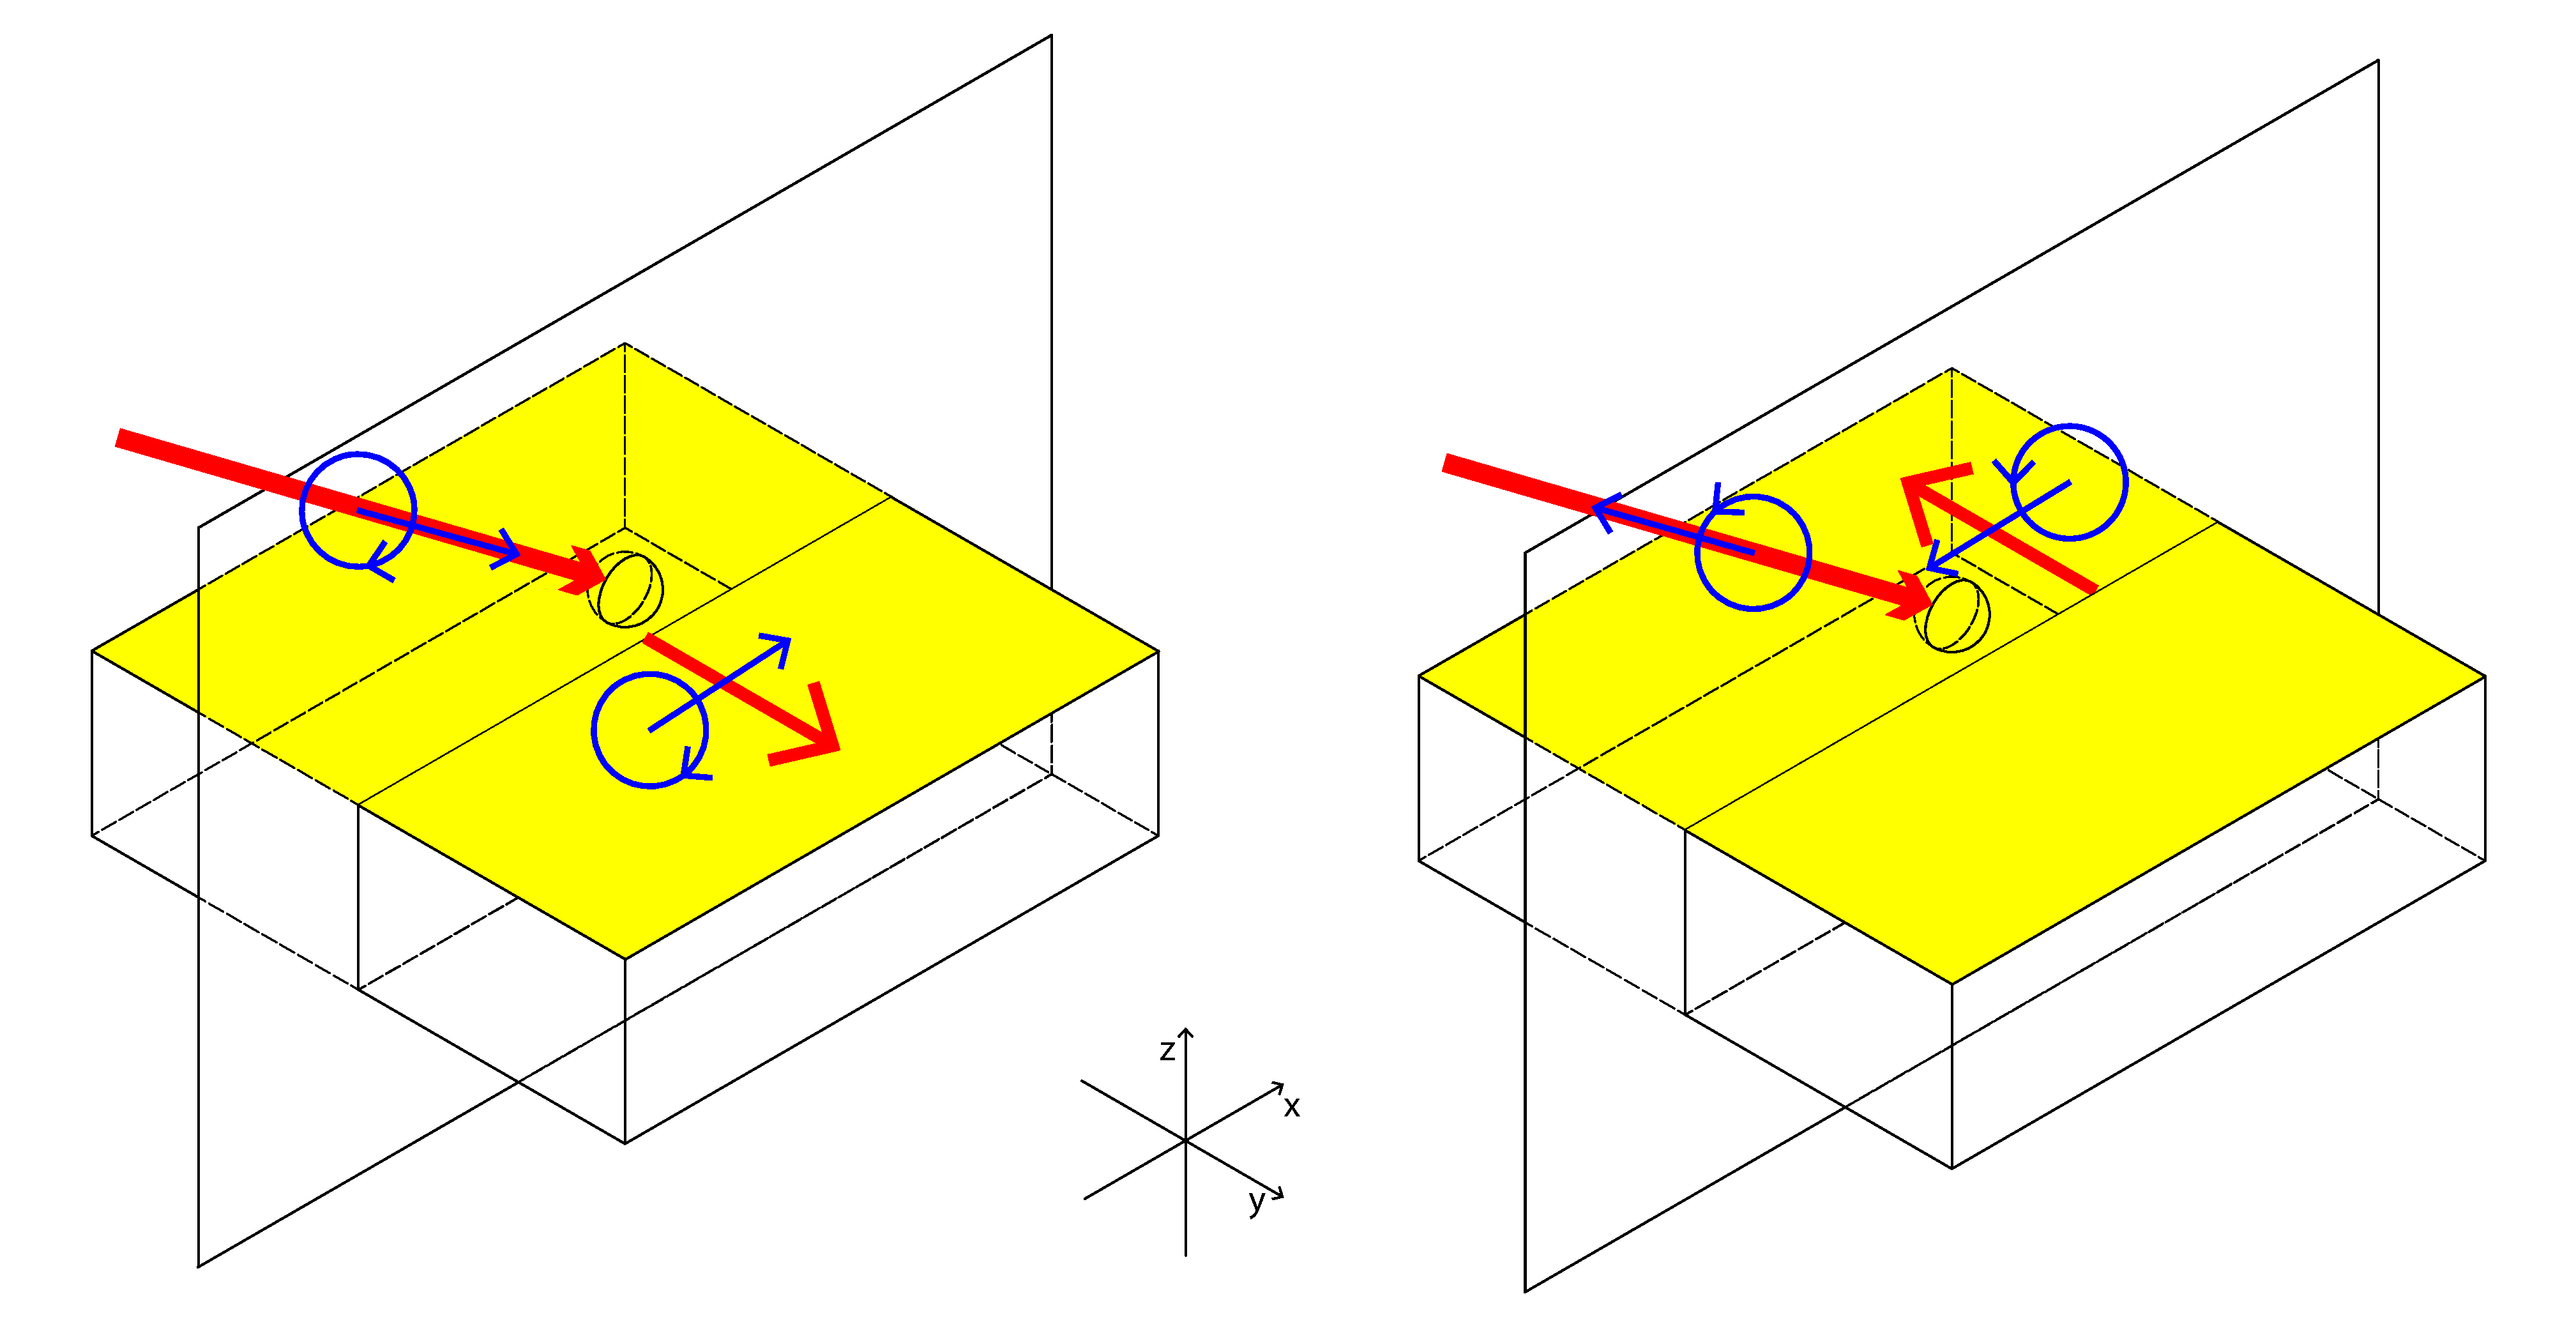
\includegraphics[width=1.0\linewidth]{figures/spin_hall_schema.pdf}
		\caption[Spin-Erhaltung PSHE]{Spin-Erhaltung beim PSHE. In blau ist jeweils der Spin des Plasmons und der anregenden Strahlung gekennzeichnet.}
		\label{fig:spin_hall_schema}
	\end{figure}
	
	
	
	\section{Messmethoden und experimenteller Aufbau}
	\subsection{Leckstrahlmikroskopie}
	In dieser Arbeit kommt ein Leckstrahlmikroskop zum Einsatz, um den PSHE experimentell nachzuweisen. Ein LRM hat gegenüber anderen Methoden zur Untersuchung plasmonischer Systeme den Vorteil, dass es rein optisch arbeitet und deswegen nicht auf aufwendige Vakuum-Technik angewiesen ist. Ein LRM nutzt aus, dass ein SPP in einem Mehrschichtsystem, wie in Abschnitt \ref{sec:leakage_radiation} erläutert, Leckstrahlung unter einem spezifischen Winkel in ein Substrat dissipiert. Als Probe wurde in dieser Arbeit ein auf ein Glassubstrat aufgedampfter Goldfilm verwendet. Das Schichtsystem besteht also aus der Abfolge Luft-Gold-Glas.
	
	Ein Defekt auf der Probe wird zunächst von der Luftseite mit einem Laser bestrahlt. An der Luft-Gold-Grenzfläche werden hierdurch SPP angeregt. Diese SPP geben nun Leckstrahlung in das Glassubstrat ab.
	Außerdem wird ein Teil des Lasers direkt transmittiert. Auf der Glasseite der Probe werden mit einem Immersionsobjektiv die Leckstrahlung und der direkt transmittierte Laser gesammelt und abgebildet.	
	Aus diesem Bild wird mit Hilfe eines 4f-Aufbaus (Abschnitt \ref{sec:fourier}) die Leckstrahlung selektiert, welche unter dem spezifischen Leckstrahlwinkel aus dem Glassubstrat ausgetreten ist. So ist es möglich, die plasmonischen Anregungen ohne Störungen des direkt transmittierten Strahls zu beobachten. Das in dieser Arbeit verwendete LRM basiert auf dem Aufbau, den \textit{Jaruschewski} im Rahmen seiner Masterarbeit \cite{Jaruschewski.2020} entwickelt hat.
	\subsubsection{Immersionsobjektiv}
	Da der Winkel, unter dem das SPP Leckstrahlung in das Glas abgibt, größer ist als der kritische Winkel für die Totalreflexion an der Grenzschicht Glas-Luft, muss für die Abbildung der Leckstrahlung ein Immersionsobjektiv verwendet werden. Ein Immersionsobjektiv nutzt ein Immersionsöl, das zwischen Objektiv und Probe aufgebracht wird. Durch die Adhäsions- und Kohäsionskräfte in dem Öl ist es möglich, dauerhaft einen kleinen Öltropfen zwischen Objektiv und Probe zu halten. In dieser Arbeit  wurde eine sogenannte homogene Immersion verwendet, dies bedeutet, dass die Brechungsindices von Deckglas, Immersionsöl und Frontlinse sehr nah beieinander liegen. Dadurch tritt an der Grenzfläche Glas-Immersionsöl für die Leckstrahlung keine Totalreflexion auf. Durch den großen Winkel, unter dem die Leckstrahlung aus der Probe austritt, ist es außerdem notwendig, dass das Objektiv einen großen maximalen Öffnungswinkel aufweist, damit die Leckstrahlung korrekt abgebildet und nicht im Inneren des Objektives absorbiert wird. Die Fähigkeit eines Objektivs, Licht unter großen Winkeln zur optischen Achse aufzunehmen, lässt sich durch die numerische Apertur $\mathrm{NA} = n\sin\theta_{max}$ beschreiben. $n$ ist hierbei der Brechungsindex des Mediums vor dem Objektiv, und $\theta_{max}$ ist der halbe maximale Öffnungswinkel des Objektivs. Die numerische Apertur berücksichtigt also, dass der Winkel eines Strahls zur optischen Achse durch Verwendung eines Mediums mit großem Brechungsindex zwischen Objektiv und Probe verkleinert werden kann. Eine große numerische Apertur bedeutet, dass das Objektiv Licht auch noch unter großen Winkeln zur optischen Achse aufnehmen kann. In dieser Arbeit wurde ein Immersionsöl mit Brechungsindex $n_{"ol} = 1.518$ und ein Immersionsobjektiv mit $\mathrm{NA} = 1.216$ verwendet. Hieraus ergibt sich ein maximaler halber Öffnungswinkel von $\theta_{max} = \arcsin(\mathrm{NA} / n_{"ol}) = 53.2^\circ > \theta_L = 43.2^\circ$. Das verwendete Immersionsobjektiv kann die Leckstrahlung also abbilden. Ferner ist das Immersionsobjektiv unendlich korrigiert. Dies bedeutet, dass die Korrekturen der Abbildungsfehler des Objektivs darauf abgestimmt worden sind, dass die Probe in der Brennweite des Objektivs steht. Wenn die Probe in der Brennweite des Objektivs steht, ist die Strahlung, welche aus dem Objektiv austritt, parallel und das Zwischenbild entsteht erst im Unendlichen. (Unter Vernachlässigung der komplexen Abbildungskorrekturen kann ein Objektiv als eine einfache Sammellinse angesehen werden.) Um dieses Zwischenbild in eine endliche Distanz zu verschieben, ist noch eine weitere Sammellinse, die Tubuslinse notwendig. Ein unendlich korrigiertes Objektiv kann auch außerhalb dieser Betriebsart verwendet werden. Allerdings treten dann zunehmend Fehler in der Abbildung auf. Der korrekte Betrieb des Objektivs kann durch die Position des Zwischenbildes hinter der Tubuslinse überprüft werden. Liegt das Zwischenbild hinter der Tubuslinse genau in deren Brennweite, so liegt die Probe in der Brennweite des Objektivs und die Abbildung des Objektives ist optimal korrigiert.\cite{Kuhl.2018}
	\subsubsection{Fourier-Optik}
	\label{sec:fourier}
	\begin{figure}[htbp] 
		\centering
		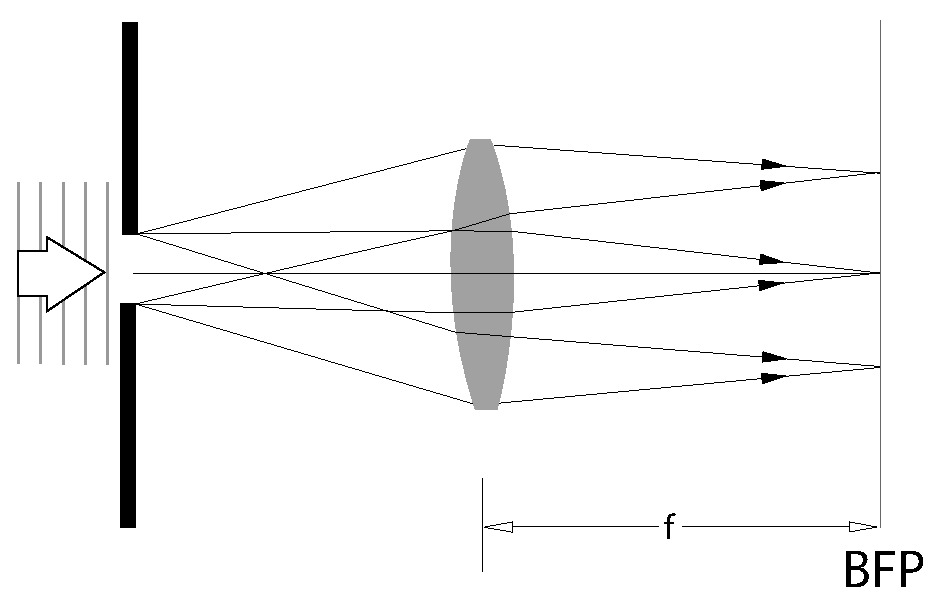
\includegraphics[width=0.5\textwidth]{figures/FourierLinse.pdf}
		\caption[Fourieroptik]{Eine Sammellinse erzeugt das Fraunhofersche Beugungsbild in ihrer hinteren Brennebene (BFP). Parallele Strahlen werden in Abhängigkeit ihres Winkels zur optischen Achse auf einem Punkt in der BFP fokussiert. Die Abbildung ist an eine Abbildung aus \cite{Hecht.2018} angelehnt.}
		\label{fig:FourierLinse}
	\end{figure}
	Da hinter der Probe nicht nur die Leckstrahlung, sondern auch die Strahlung des direkt transmittierten Strahls zu beobachten ist, ist es notwendig, die Leckstrahlung zu selektieren. Die Leckstrahlung tritt dank der notwendigen Phasenanpassung nur unter einem charakteristischen Winkel zur optischen Achse \eqref{eq:phase_condition} aus der Probe aus. Daher ist es möglich, die Leckstrahlung durch ihren Emissionswinkel zu identifizieren. Hierfür ist die Fourier-Optik nützlich. Eine Sammellinse besitzt die Eigenschaft, in  der hinteren Brennebene (eng. Back Focal Plane BFP) ein winkelaufgelöstes Bild von der Strahlung, die sie erreicht, zu erzeugen\cite{Hecht.1996}. Die Position eines Lichtstrahls in der BFP ist also nur von dem Winkel des Strahls zur optischen Achse, nicht aber von der absoluten Position des Strahls vor der Linse abhängig. So ist es möglich, gezielt bestimmte Emissionswinkel in der BFP aus dem Bild herauszufiltern. Dieses winkelaufgelöste Bild kann auch als eine räumliche Fouriertransformation der Feldstärkeverteilung an der beobachteten Struktur aufgefasst werden. 
	
	\paragraph{4f-Aufbau}
	In dieser Arbeit wird für diese optische Filterung ein $4f$-Aufbau verwendet. Ein $4f$-Aufbau besteht aus zwei Linsen mit der Brennweite $f$, die im Abstand $2f$ zueinander angeordnet werden. Die beiden Linsen werden so positioniert, dass sich im Abstand $f$ von der ersten Linse das Zwischenbild des Immersionsobjektivs befindet. Zwischen den beiden Linsen entsteht nun ein winkelaufgelöstes Fourierbild; Dieses wird durch die numerische Apertur des Immersionsbildes scharf begrenzt.  In diesem winkelaufgelösten Fourierbild kann nun gezielt ein Teil des Fourierspektrums (d.h. der Strahlung, die unter einem bestimmten Winkel zur optischen Achse aus der Probe ausgetreten ist) herausgefiltert werden. Die zweite Linse erzeugt nun aus diesem gefilterten Fourierspektrum wieder das Ortsbild. Dieses besteht nun nur noch aus den ausgewählten Fourierkomponenten. Der $4f$-Aufbau ist schematisch in Abbildung \ref{fig:aufbau_schema} erläutert. In dieser Arbeit wurde so der direkt transmittierte Strahl aus der optischen Abbildung eliminiert.
	\subsection{Einstellung der Polarisation des Lasers}
	\label{sec:cntr_pol}
	Um den optischen Spin-Hall-Effekt nachweisen zu können, ist es notwendig, die Polarisation des Anregungslasers zu kontrollieren. Hierfür wurden ein Polfilter und eine $\lambda /4$-Verzögerungsplatte verwendet. Der in dieser Arbeit verwendete He-Ne-Laser der Firma \textit{Thorlabs} ist linear polarisiert. 
	\paragraph{Polarisationsfilter}	
	Um die Polarisationsebene des Lasers präzise festzulegen, wurde ein linearer Polfilter verwendet. Ein beliebiger Polarisationszustand lässt sich immer durch eine Überlagerung von zwei senkrecht aufeinander stehenden linearen Polarisationen darstellen. Ein Polfilter transmittiert nun nur Licht, welches entlang einer festgelegten Achse linear polarisiert ist. Die anderen Polarisationsrichtungen werden absorbiert oder reflektiert. Ein Polfilter kann also aus einer beliebigen Polarisation linear polarisiertes Licht erzeugen. Der  Polfilter wurde nach dem letzten Spiegel des optischen Aufbaus positioniert, da ein Spiegel im Allgemeinen unterschiedliche Reflektivitäten für EM-Strahlung aufweist, je nachdem, ob diese Strahlung senkrecht oder vielmehr parallel zur Einfallsebene des Strahls auf den Spiegel polarisiert ist. Der Filter wurde auf eine Polarisation parallel zur Einfallsebene eingestellt und der Laser dann so entlang der optischen Achse gedreht, dass die gemessene Intensität hinter dem Polfilter maximal ist. So entsteht hinter dem Polfilter unabhängig  von der exakten ursprünglichen Polarisation des Lasers $p$-polarisiertes Licht.
	\paragraph{Verzögerungsplättchen}
	Mit einem Verzögerungsplättchen lässt sich die Polarisation einer einfallenden Welle verändern. Eine EM-Welle lässt sich immer als Überlagerung von zwei linear senkrecht zueinander polarisierten Wellen beschreiben. Diese beiden senkrecht aufeinander stehenden Polarisationen sind im Allgemeinen zueinander phasenverschoben. Das Funktionsprinzip eines Verzögerungsplättchens besteht darin, die relative Phasenverschiebung zwischen diesen beiden Polarisationen zu verändern. So kann man mit einem geschickt gewählten Verzögerungsplättchen aus jeder beliebigen Ausgangspolarisation in einen beliebigen anderen Polarisationszustand wechseln. Ein Verzögerungsplättchen weist immer eine schnelle und eine langsame Achse auf. Diese beiden Achsen stehen senkrecht aufeinander. Die Phasenverschiebung zwischen zwei EM-Wellen, von denen die eine entlang der langsamen Achse und die andere entlang der schnellen Achse polarisiert ist, stellt eine charakteristische Größe ($\Delta\Phi$) des jeweiligen Verzögerungsplättchens dar. Physikalisch  werden Verzögerungsplättchen durch doppelbrechende Kristalle realisiert. Die jeweilige Phasendifferenz ist hierbei von der Dicke des doppelbrechenden Kristalls und von den Brechungsindizes der langsamen und der schnellen Kristallachse abhängig. Wenn diese Größen so dimensioniert sind, dass die Phasendifferenz zwischen den beiden Polarisationen, die eine EM-Welle beim Durchgang durch das Plättchen erfährt, $\Delta \Phi = \pi /4 $ ist, spricht man von einem  $\lambda /4$-Verzögerungsplättchen. Diese Phasendifferenz ist immer an eine bestimmte Wellenlänge angepasst.  Ein $\lambda /4$-Verzögerungsplättchen kann aus linear polarisiertem Licht zirkular polarisiertes Licht erzeugen, wenn eine der beiden Kristallachsen eine Orientierung von 45° zur ursprünglichen Polarisationsachse des Lasers aufweist \cite{Hecht.2018}. Diese Eigenschaft wurde in dieser Arbeit ausgenutzt. In Abbildung \ref{fig:polarisationlambda} ist die Polarisation hinter dem Verzögerungsplättchen in Abhängigkeit der relativen Orientierung vom Polfilter zum $\lambda /4$-Verzögerungsplättchen dargestellt. 
	\begin{figure}
		\centering
		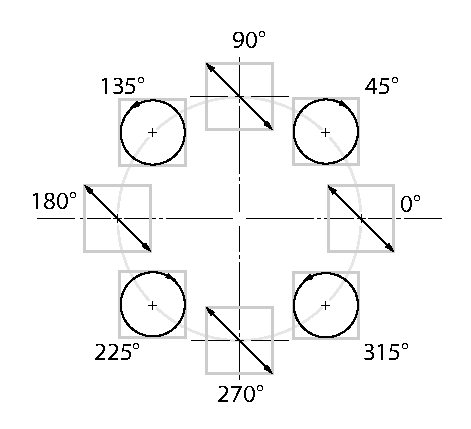
\includegraphics[width=0.5\linewidth]{figures/Polarisation_lambda}
		\caption[Polarisation $\lambda/4$-Plättchen]{Die Abbildung zeigt die Polarisation abhängig von der relativen Orientierung zwischen $\lambda/4$-Plättchen und Polfilter hinter dem $\lambda/4$-Plättchen.}
		\label{fig:polarisationlambda}
	\end{figure}
	
	\subsection{Details des optischen Aufbaus}
	In dieser Arbeit wurde der Aufbau von \textit{Jaruschewski} \cite{Jaruschewski.2020} in einigen Details verbessert und umgerüstet, so dass der Laser auch unter schrägem Einfall auf die Probe gerichtet werden kann. Die verwendeten Komponenten sind detailliert in Anhang \ref{tab:components} aufgelistet. Der Aufbau ist in Abbildung \ref{fig:aufbau_schema} schematisch dargestellt. Als Anregungslaser wurde ein He-Ne-Dauerstrich-Laser der Firma \textit{Thorlabs} mit einer Leistung von $P = 35 \,\mathrm{mW}$ und Wellenlänge $\lambda = 633\,\mathrm{nm}$ verwendet. Der Laser ist linear polarisiert.
	\begin{figure}
		\centering
		\begin{subfigure}[b]{0.9\textwidth}		
			\centering
			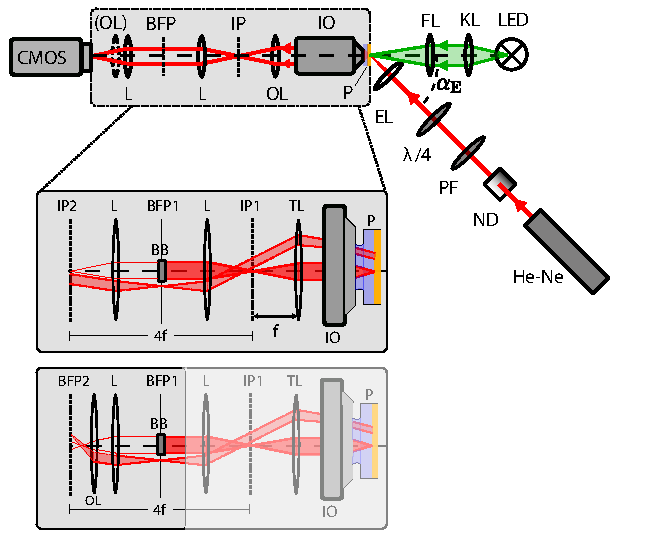
\includegraphics[width=0.9\textwidth]{figures/Aufbau_Schema.pdf}
			\caption{Schematischer Aufbau}			
			\label{fig:aufbau_schema}
		\end{subfigure}
		\vfil
		\begin{subfigure}[b]{0.9\textwidth} 
			\centering
			\includegraphics[width=0.9\textwidth]{figures/aufsicht_aufbau_anotated.jpg}
			\caption{Foto des Aufbau}
			\label{fig:aufsicht_aufbau_anotated}
		\end{subfigure}
		\caption[Versuchsaufbau]{Die Komponenten des Aufbaus sind: He-Ne-Laser (He-Ne), Neutraldichtefilter (ND), Polarisationsfilter (PF), Verzögerungsplättchen ($\\lambda/4$), Einkoppel-Linse (EL), Probe, Immersionsobjektiv (IO), Linse 2 (L2), Image-Filter (IF), Linse 1 (L1), Beam-Block (BB), Linse 2 (L2), optionale Linse (OL), CMOS-Sensor (CMOS). Außerdem ist auch noch eine LED-Hintergrundbeleuchtung verbaut. In rot ist schematisch der Strahlengang des Lasers eingezeichnet. Die Abbildung des schematischen Aufbaus ist an eine Abbildung aus \cite{Jaruschewski.2020} angelehnt.}
		\label{fig:Aufbau}
	\end{figure}
	\subsubsection{Optische Komponenten und ihre Funktion}
		In diesem Abschnitt werden alle verwendeten optischen Komponenten benannt (in Strahlreihenfolge), und die zugehörige Funktion wird kurz erläutert. Die Komponenten sind in Abbildung \ref{fig:Aufbau} dargestellt.
		\begin{itemize}
			\item \textbf{Neutraldichtefilter (ND)} dient der Abschwächung des Lasers, um eine Überbelichtung des CMOS-Sensors zu verhindern.
			\item \textbf{Polfilter (PF)} dient der Kontrolle der Polarisation des Lasers (siehe Abschnitt \ref{sec:cntr_pol}).
			\item $\boldsymbol{\lambda / 4}$\textbf{-Plättchen (}$\boldsymbol{\lambda / 4}$\textbf{)} dient der Kontrolle der Polarisation des Lasers (siehe Abschnitt \ref{sec:cntr_pol}).
			\item \textbf{Einkoppellinse (EL)} dient der Fokussierung des Lasers auf die Probe, um hohe Intensitäten zu erreichen und möglichst gezielt einen Defekt zu beleuchten.
			\item \textbf{Probe (P)} Auf der Gold-Glas-Probe werden die SPP angeregt.
			\item \textbf{Immersionsobjektiv (IO)} dient der Abbildung der Leckstrahlung.
			\item \textbf{Tubuslinse (TL)} dient der Abbildung der Leckstrahlung.
			\item \textbf{Image-Block (IB)} dient der Filterung des Ortsbildes, so dass nur Leckstrahlung, die aus einem kleinen Bereich der Probe stammt, abgebildet wird.			
			\item \textbf{Linse 1 (L1)} ist Teil des 4f-Systems (siehe Abschnitt \ref{sec:fourier}).
			\item \textbf{Beam-Block (BB)} dient der Filterung der BFP. Der BB sperrt den direkt transmittierten Strahl.			
			\item \textbf{Linse 2 (L2)} ist Teil des 4f-Systems (siehe Abschnitt \ref{sec:fourier}).
			\item \textbf{Optionale Linse (OL)} kann aus dem Aufbau entfernt werden und wird verwendet, um zwischen orts- und winkelaufgelöstem Bild zu wechseln.
			\item \textbf{CMOS Sensor (CMOS)}  dient der Aufzeichnung des Bildes. Ist über Ethernet mit dem Computer verbunden.			
		\end{itemize}
		Um die Fokussierung der Probe zu erleichtern, wurde außerdem eine LED-Hintergrundbeleuchtung verwendet. Das Licht der LED wurde mit einer Sammellinse kollimiert und mit einer weiteren Linse FL $f_{\mathrm{FL}}=50\mathrm{mm}$ auf die  Probe fokussiert. Diese Linse wurde bei Bedarf mit einer Magnetsäule an der richtigen Stelle vor der Probe positioniert.
		
	\subsubsection{Veränderungen des vorhandenen Aufbaus}
	\paragraph{Einkoppellinse}
	Aus geometrischen Gründen war es nicht mehr möglich, den Laser mit einem Objektiv bei streifendem Einfall auf die Probe zu fokussieren, da sonst das Objektiv mit der Probe kollidieren würde. Stattdessen wurde eine Sammellinse als Einkoppellinse (EL) verwendet mit $f_{\mathrm{EL}}= 30\mathrm{mm}$. Die Wahl der Brennweite der Einkoppellinse ist ein Kompromiss: Je kleiner die Brennweite ist, desto kleiner lässt sich der Laser fokussieren. Wenn die Brennweite allerdings zu klein ist, kollidiert die Linsenhalterung mit der Probe. Mit kleinerer Brennweite sind also nur kleinere Einfallswinkel zur Probennormale möglich. Um trotzdem eine möglichst kleine Brennweite verwenden zu können, wurde eine sehr kompakte Linsenhalterung verwendet. Diese Halterung wurde über einen Querarm an einer xyz-Verfahreinheit montiert, so dass man die Linse in allen drei Raumrichtungen verfahren kann. Dies ist wichtig, um den Laser gezielt auf den Punkt zu fokussieren, an welchem die optische Achse die Probe schneidet. Dieser Aufbau ist in Abbildung \ref{fig:linsenhalterung} gezeigt.
	\begin{figure}
		\centering
		\begin{subfigure}[b]{0.4\textwidth}
			\centering
			\includegraphics[width=\textwidth]{figures/Einkoppellinse.jpg}
			\caption{Querarm}
			\label{fig:querarm}
		\end{subfigure}
		\hfill
		\begin{subfigure}[b]{0.4\textwidth}
			\centering
			\includegraphics[width=\textwidth]{figures/Kollision_Einkoppellinse.jpg}
			\caption{Kollision Linse mit Probe}
			\label{fig:kollision}
		\end{subfigure}
		\caption[Einkoppellinse-Halterung]{Diese Abbildungen zeigen die Linsenhalterung, welche über einen Querarm an einer xyz-Verfahreinheit montiert ist, und die Kollision zwischen Linsenhalterung und Probe}
		\label{fig:linsenhalterung}
	\end{figure}
	
	\paragraph{Probenhalterung}
	Die Probenhalterung des alten Aufbaus wies das Problem auf, dass die senkrechte Ausrichtung der Probe zur optischen Achse nur grob per Auge erfolgen konnte. Dadurch war beim Verfahren der Probe ein ständiges Nachfokussieren erforderlich. Außerdem fehlte der Halterung die ausreichende Stabilität, was die Fokussierung zusätzlich erschwerte. Daher wurde im Rahmen dieser Arbeit eine neue Probenhalterung entwickelt, konstruiert und die zentrale Werkstatt im Physikzentrum mit der Fertigung beauftragt. Eine technische Zeichnung der Probenhalterung ist im Anhang zu finden \ref{fig:tz_probenhalter}. Diese Probenhalterung behebt die Schwachstellen der alten und hat außerdem einen Anschlag für die Probe, so dass es nun prinzipiell möglich ist, anhand der Skalen an den Mikrometerschrauben der Verfahreinheit Koordinaten abzulesen. So wird ermöglicht, trotz eines Probenwechsel später wieder die gleichen Orte auf der Probe anzufahren.
	\begin{figure}[htbp] 
		\centering
		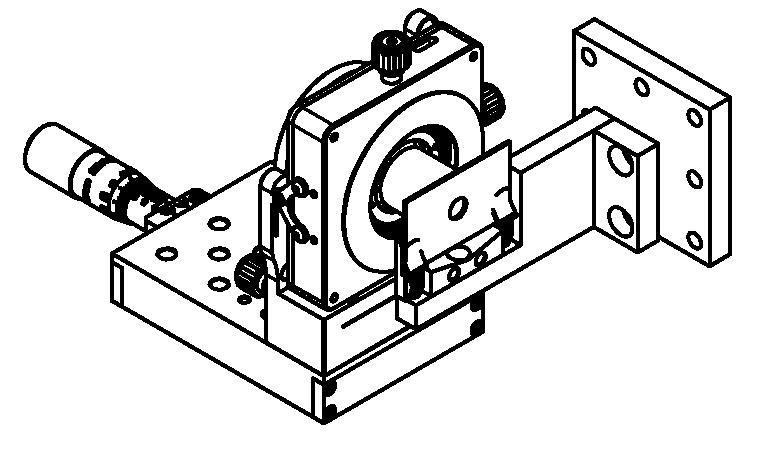
\includegraphics[width=0.5\textwidth]{figures/Probenhalter.pdf}
		\caption[Probenhalterung]{Probenhalter mit montierter Probe vor dem Immersionsobjektiv}
		\label{fig:probenhalter}
	\end{figure}
	\paragraph{Cage-System}
	Sämtliche Optiken hinter dem Immersionsobjektiv wurden in ein Cage-System der Firma \textit{Thorlabs} integriert (Abbildung \ref{fig:cage_system}). Das Cage-System besteht aus quadratischen Halterungen, die in ihren Eckpunkten Bohrungen haben, durch welche sich Edelstahlstäbe schieben lassen. Diese Fixierung der Halterungen an vier Punkten verhindert ein Verkippen der Linsen entlang der optischen Achse. Die Halterungen können entlang der optischen Achse auf den vier Eckstäben verschoben werden. Für die  Linsen TL, L1, L2 wurden xy-Halter verwendet, die senkrecht zur optischen Achse mit feinen Justierschrauben sehr genau verstellt werden können. Im Laufe dieser Arbeit hat sich herausgestellt, dass diese sehr feine Justierung nicht notwendig gewesen wäre. Die Tubuslinse TL des Herstellers \textit{Zeiss} ist in einem Halter mit einem $M32\times0.5$ Gewinde montiert. Eine technische Zeichnung der Tubuslinse ist in Abbildung \ref{fig:tubelensetz} zu finden. Für dieses Gewinde stellt \textit{Thorlabs} keine Komponenten her, deswegen war ein Adapter notwendig. Eine technische Zeichnung dieses Adapters ist in Abbildung \ref{fig:tz_adapter} zu finden. Die optionale Linse OL wurde mit einer Magnethalterung in das Cage-System eingebaut. Diese Halterung ermöglicht es, die Linse sehr einfach zu entfernen und so zwischen der Darstellung der Image-Plane und der Backfocal-Plane zu wechseln. Außerdem wurde die OL in einem längeren Gewindetubus montiert, so dass ein präzises Verfahren der Linse entlang der optischen Achse möglich ist. Dies ist notwendig, um die BFP exakt zu fokussieren. Ist die richtige Position der OL einmal bestimmt, kann der Gewindetubus mit einem Gewindering gekontert werden. Auch der CMOS-Sensor der Firma \textit{Allied-Vision} wurde in das Cage-System integriert. Hierfür war ein Adapter von der Kameraobjektiv-Gewindenorm \textit{C-Mount} auf die Gewindenorm \textit{SM-2} des Cage-System Herstellers \textit{Thorlabs} notwendig. Dieser Adapter wurde im Rahmen dieser Arbeit entwickelt und konstruiert und dann von \textit{Sönke Harm} gefertigt. Eine technische Zeichnung des Cage-Systems ist in Abbildung \ref{fig:tz_cage_system}und eine des Adapters in \ref{fig:tz_adapter} zu finden. Der Beam-Block (BB) und der Image-Filter (IF) sind mit Magnetsäulen auf dem optischen Tisch befestigt.
	\begin{figure}[htbp] 
		\centering
		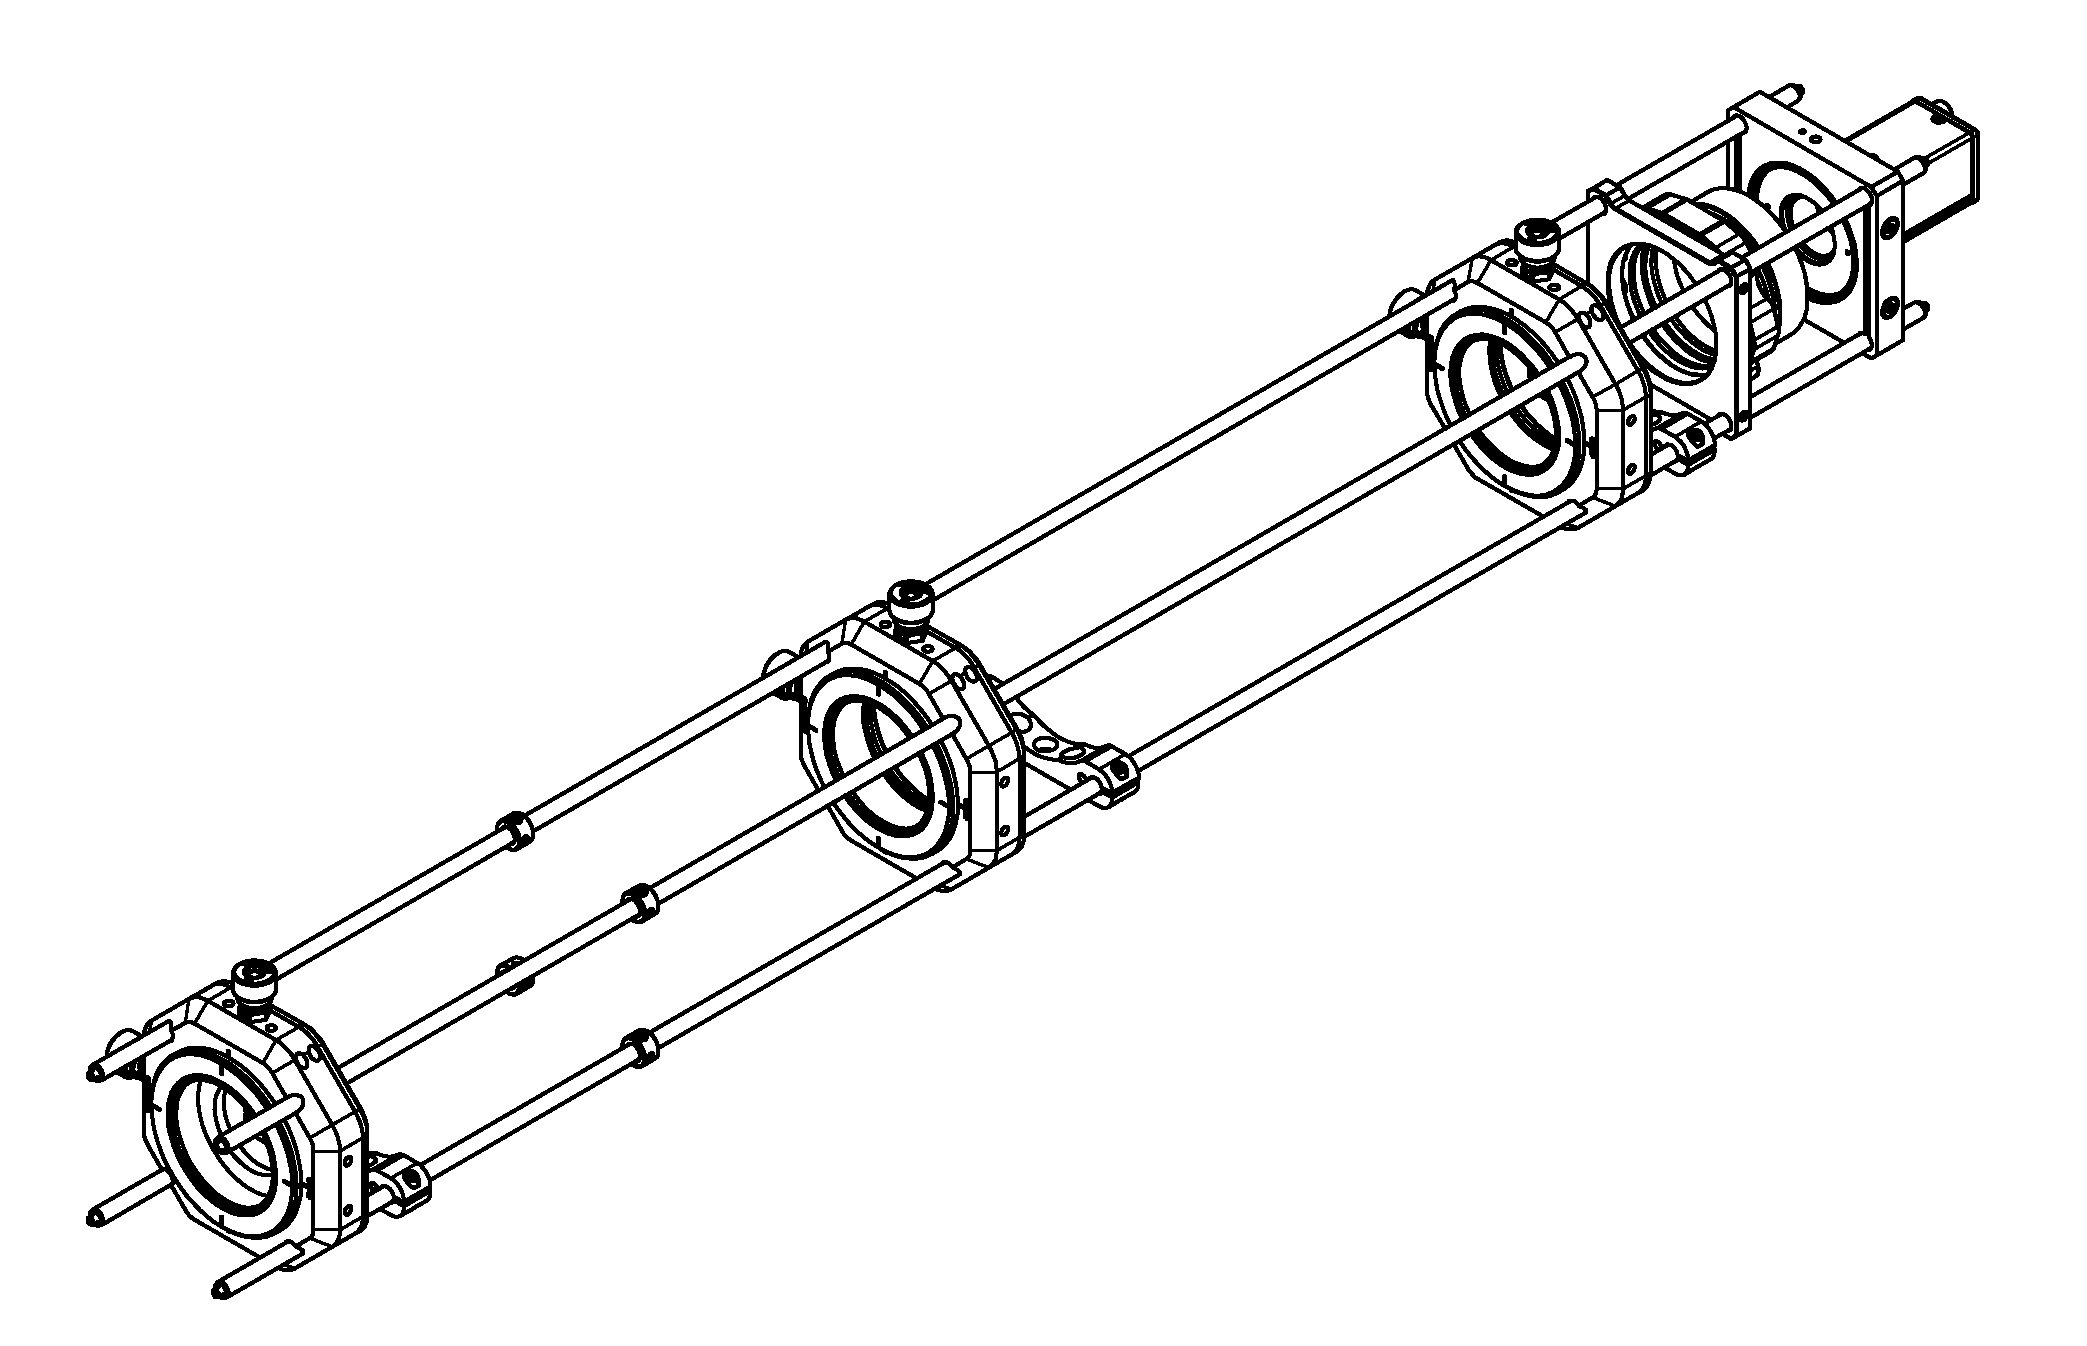
\includegraphics[width=0.7\textwidth]{figures/Cage_System.pdf}
		\caption[Cage-System]{Tubuslinse, 4f-System, optionale Linse und CMOS im Cage-System}
		\label{fig:cage_system}
	\end{figure}	
	\subsection{Probe}
	Die ersten Messungen dieser Arbeit wurden mit Proben, die noch durch die Messungen von \textit{Jaruschewski} \cite{Jaruschewski.2020} vorhanden waren, durchgeführt. Da diese Proben jedoch auch auf der Goldseite mit Immersionsöl kontaminiert waren, wurden später neue Proben verwendet. Diese Proben wurden von Till Leißner in S\o nderborg hergestellt. Hierfür wurden Deckgläser der Firma \textit{Carl Zeiss} mit einem Brechungsindex von $n_{\mathrm{Glas}}= 1.52$ verwendet. Die Deckgläser wurden mit einer $d_{\mathrm{Gold}} = 50\mathrm{nm}$ dicken Goldschicht bedampft. Die Deckgläser haben eine Dicke von $d_{\mathrm{Glas}} = 170 \mathrm{\mu m}$. Als Anregungsstruktur wurden Defektstellen verwendet. Die Proben wurden in kleine Edelstahlbleche (Technische Zeichnung \ref{fig:tz_probenblech}) eingeklebt, welche wiederum in die Probenhalterung passen. Damit die Proben auf der Goldseite nicht mit Immersionsöl kontaminiert werden, wurden sie mit einem Epoxid-Kleber in die Edelstahlbleche abdichtend eingeklebt.
	\begin{figure}
		\centering
		\begin{subfigure}[b]{0.4\textwidth}
			\centering
			\includegraphics[width=\textwidth]{figures/Probe_Vorderseite.jpg}
			\caption{Goldseite}
			\label{fig:probe_vorderseite}
		\end{subfigure}
		\hfill
		\begin{subfigure}[b]{0.4\textwidth}
			\centering
			\includegraphics[width=\textwidth]{figures/Probe_Rueckseite.jpg}
			\caption{Glasseite}
			\label{fig:probe_rueckseite}
		\end{subfigure}
		\caption[Eingeklebte Probe]{Die Bilder zeigen die in das Edelstahlblech eingeklebte Probe. In rot ist die Verklebung markiert. Hierbei war darauf zu achten, dass die Klebung dicht ist, so dass kein Öl von der Glasseite auf die Goldseite laufen kann.}
		\label{fig:probe}
	\end{figure}
	\subsection{Justage des Aufbaus}
	Die allgemeine Justage des LRM verlief - bis auf die Justage des Lasers auf die Probe - wie von \textit{Jaruschewski} \cite{Jaruschewski.2020} beschrieben. Dieses war durch den notwendigen schrägen Einfall des Lasers auf die Probe deutlich erschwert. Die Justage erfolgte mit montierter Probe. Zunächst wurde die Probe mit Hilfe der Hintergrundbeleuchtung in den korrekten Abstand zum IO gebracht (im korrekten Abstand ist das Bild der Probe scharf zu sehen). Als nächstes wurde der Laser mit zwei Spiegeln grob in dem erwünschten Winkel auf die Probe justiert. Danach wurden Einkoppellinse, $\lambda/4$-Plättchen und Polfilter in den Strahlgang gestellt. Die Feinjustierung des Lasers auf die Probe wurde nun durch das Verschieben der Einkoppellinse durchgeführt. Hierbei ist es hilfreich, den Strahl durch das Verfahren der EL entlang der optischen Achse etwas zu de-fokussieren, so dass man die Randbereiche des Strahls über den CMOS-Sensor in der Image-Plane auch schon sehen kann, wenn der Strahl noch nicht exakt die optische Achse trifft. Sobald ein Teil des Strahls in der Image-Plane detektiert worden ist, wird er durch weiteres Bewegen der Linse zentriert und dann schrittweise weiter fokussiert. Durch das Verkippen der Einkoppellinse zum Laser wandert der Strahl beim Fokussieren des Lasers auf der Probe aus. Das Verkippen der Linse wird behoben, sobald der Laser optimal fokussiert ist. Hierfür wird der Laser durch die beiden Spiegel sukzessive so einjustiert, dass der Spot auf der Probe beim Defokussieren des Lasers nicht mehr wandert.
	\subsection{Bestimmung der Polarisation des Anregungslasers}
	Für die Kontrolle der Polarisation des Anregungslasers ist es von entscheidender Bedeutung, dass der ursprüngliche Polarisationszustand bekannt ist. Außerdem zeigen die folgenden Messungen, dass die vom Hersteller angegebene Orientierung des $\lambda/4$-Plättchens und des Polfilters grob stimmen. Die Messungen sind außerdem ein starkes Indiz dafür, dass sowohl das $\lambda/4$-Plättchen als auch der Polarisationsfilter ordnungsgemäß funktionieren. Die folgenden Ausführungen sind also für das Verständnis der weiteren Arbeit nicht zwingend erforderlich, schließen aber einige wichtige Fehlerquellen aus. Außerdem zeigt die folgende Messung, dass der Polfilter der in dem Hauptaufbau vor dem $\lambda / 4$-Plättchen verwendet wurden ist, um die Polarisation vor dem $\lambda / 4$-Plättchen zu definieren, notwendig ist. 
	\subsubsection{Jones-Formalismus}
	Der Jones-Formalismus ist ein Formalismus, der es ermöglicht, die Polarisation von elektromagnetischer Strahlung mathematisch zu beschreiben. Das elektrische Feld einer monochromatischen ebenen Welle lässt sich durch folgenden Ausdruck beschreiben:
	\begin{equation}
		\vec{E}(z, t) = \underbrace{\begin{pmatrix}E_x \\ E_y\end{pmatrix}}_{\vec{J}} \exp(i(kz-\omega t))
	\end{equation}
	Hierbei ist $\vec{J} := \begin{pmatrix}E_x \\ E_y\end{pmatrix}$ der aus den beiden komplexen Zahlen $E_x, E_y$ bestehende Jones-Vektor. Der Jones-Vektor beschreibt also die Amplitude und das Phasenverhältnis der beiden Feldkomponenten und charakterisiert den Polarisationszustand der EM-Welle somit vollständig. Der Jones-Vektor wird also durch die vier reellen Parameter $\Re\{E_x\}, \Im\{E_x\}, \Re\{E_y\}, \Im\{E_y\}$ vollständig bestimmt. Es gibt neben diesen Parametersatz auch noch weitere Kombination von vier Parametern, die den Polarisationzustand vollständig beschreiben. (Basiswechsel des Jones-Vektors)Beispielsweise die Parameter...
	Ein beliebiges optisches Element, dass den Polarisationzustand einer EM-Welle beinflusst lässt sich nun durch eine komplexe $2 \times 2$-Jones-Matrix $\boldsymbol{M}$ beschreiben. Wenn die EM-Welle vor dem optischen Element den durch den Jones-Vektor $\vec{J}$ beschriebenen Polarisationszustand hat, hat sie nach dem Durchgang durch das optischen Element den Polarisationszustand:
	\begin{equation}
		\vec{J}^\prime = \boldsymbol{M} \vec{J}  =  
		\begin{pmatrix}
			M_{11} & M_{12} \\
			M_{21} & M_{22}
		\end{pmatrix}
		\begin{pmatrix}
			J_x \\
			J_y
		\end{pmatrix} = 
		\begin{pmatrix}
			M_{11} J_x + M_{12} J_y \\
			M_{21} J_x + M_{22} J_y
		\end{pmatrix}		
	\end{equation}
	Unterschiedliche optische Elemente lassen sich nun durch verschiedene Jones-Matrizen beschreiben. So ist die Jones-Matrix eines in $x$-Richtung orientierten Polfilters beispielsweise:
	\begin{equation}
		\boldsymbol{M}_{\mathrm{PF}} = \begin{pmatrix}
		1 & 0 \\
		0 & 0
	\end{pmatrix}
	\end{equation}
	oder eines $\lambda / 4$-Plättchens mit schneller Achse entlang der $x$-Richtung orientiert:	
	\begin{equation}
		\boldsymbol{M}_{\mathrm{\lambda / 4}} = \dfrac{1}{\sqrt{2}}\begin{pmatrix}
			1-i & 0 \\
			0 & 1+i
		\end{pmatrix}
	\end{equation}
	Die Drehung eines optischen Elements lässt sich durch das Anwenden einer Rotationsmatrix auf die Jones-Matrix ausdrücken:
	\begin{equation}
		\boldsymbol{M}(\Phi) = \boldsymbol{R}(\Phi)\boldsymbol{M}\boldsymbol{R}(-\Phi)
	\end{equation}
	mit der Rotationsmatrix:
	\begin{equation}
		\boldsymbol{R}(\Phi) = \begin{pmatrix}
			\cos\Phi & - \sin\Phi \\
			\sin\Phi & \cos\Phi
		\end{pmatrix}
	\end{equation}
	\paragraph{Bestimmung der Polarisation des Anregungslasers mit Hilfe eines Jones-Polarimeter}
	Ein Polarimeter ist eine Apparatur, die eine vollständigen Bestimmung der Polarisation von einer EM-Welle ermöglicht. Eine Realisierung eines Polarimeters ist ein Jones-Polarimeter. Dieses besteht in Strahlreihenfolge aus einem $\lambda / 4$ Plättchen, einem Polfilter und einem Leistungsmessgerät (Abbildung \ref{fig:polarimeter}). Um nun den Jones-Vektor $\vec{J}$ von einer monochromatischen ebenen Welle mit Hilfe des Jones-Polarimeters zu bestimmen, wird die Leistung in Abhängigkeit von der Orientierung $\alpha_{\lambda/4}$ des $\lambda / 4$-Plättchens gemessen: $P = P(\alpha_{\lambda/4})$. Die Form dieses Leistungsverlaufes hängt nun nur von dem ursprünglichen Polarisationszustand der EM-Strahlung ab. Um nun aus $P(\alpha_{\lambda/4})$ die Komponenten des Jones-Vektor $\vec{J}$ zu rekonstruieren, wurde das Experiment mit einem \textit{Python}-Skript simuliert. Hierfür wurde der oben Beschriebene Jones-Formalismus genutzt. Der Polarisationszustand hinter dem Polarimeter $\vec{J}^\prime$ lässt sich durch folgenden Ausdruck berechnen:
	\begin{equation}
		\vec{J}^\prime = \boldsymbol{M}_\mathrm{PF} \boldsymbol{R}(\alpha_{\lambda/4})\boldsymbol{M}_{\lambda / 4}\ \boldsymbol{R}(-\alpha_{\lambda/4})\vec{J}
	\end{equation}
	Die Intensität und damit auch die Leistung bei konstantem Strahlquerschnitt, die an dem Leistungsmessgerät ankommt ist hierbei proportional zum Betragsquadrat des Jones-Vektors:
	\begin{equation}
		P(\vec{J}^\prime) \propto \left|\vec{J}^\prime\right|^2
	\end{equation}
	Die theoretisch erwartete Leistung $P$, die an dem Leistungsmessgerät erwartet wird, ergibt sich also in Abhängigkeit von $\alpha_{\lambda/4}$ und $\vec{J}$ zu:
	\begin{equation}
		P(\alpha_{\lambda/4}, \vec{J}) = \left|\boldsymbol{M}_\mathrm{PF} \boldsymbol{R}(\alpha_{\lambda/4})\boldsymbol{M}_{\lambda / 4}\ \boldsymbol{R}(-\alpha_{\lambda/4})\vec{J}\right|^2 \cdot \mathrm{const.}
		\label{eq:simulation_polarimeter}
	\end{equation}
	Diese Funktion kann nun mit den Komponenten von $\vec{J}$ als Parameter mit Hilfe der Methode der kleinsten quadratischen Abweichung (engl. \textit{least square fit}) an die Messdaten angepasst werden. Die resultierenden Fit-Parameter sind dann die Komponenten des ursprünglichen Jones-Vektors $\vec{J}$. Dieser Fit an die Messdaten und die resultierende Polarisations-Ellipse ist in Abbildung \ref{fig:graphpolarimeter} dargestellt. In der Abbildung ist zu erkennen, dass die Messdaten sehr gut mit der Simulation übereinstimmen. Dies ist ein starkes Indiz für die korrekte Funktionsweise der Komponenten. Allerdings zeigt die Messung auch, dass der Laser nicht rein linear Polarisiert ist. Hierfür ist die Elliptizität $\epsilon$ der Polarisation ein gutes Maß:
	\begin{equation}
		\epsilon = \arctan\left(\dfrac{a}{b}\right)
	\end{equation}
	Hierbei ist $a$ die große Halbachse der Polarisationsellipse und $b$ die kleine Halbachse der Polarisationsellipse. Die Elliptizität des Lasers wurde in dieser Arbeit auf $\epsilon = 0.1 $ bestimmt. Durch diese Abweichungen des Lasers von einer rein linearen Polarisation, war es notwendig die Polarisation des Lasers vor dem $\lambda /4$-Plättchen im Hauptaufbau durch einen Polfilter festzulegen.
	\begin{figure}
		\centering
		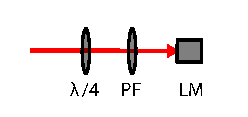
\includegraphics[width=0.5\linewidth]{figures/Polarimeter}
		\caption[Jones-Polarimeter]{Die Abbildung zeigt den schematischen Aufbau eines Jones-Polarimeter. Die Komponenten in Strahlreihenfolge sind: Helium-Neon-Laser (\textbf{He-Ne}), $\lambda/4$-Plättchen ($\boldsymbol{\lambda / 4}$), Polfilter (\textbf{PF}), Leistungsmessgerät(\textbf{LM}). Das $\lambda/4$-Plättchen ist kann um die optische Achse rotiert werden.}
		\label{fig:polarimeter}
	\end{figure}
	\begin{figure}
		\centering
		\includegraphics[width=0.7\linewidth]{figures/graph_polarimeter}
		\caption[Polarimeter Simulation]{Diese Abbildung zeigt die Messdaten einer Messung mit dem Jones-Polarimeter. Der untere Teil der Abbildung zeigt die gemessene Leistung $P(\alpha_{\lambda /4}$. Die blauen Kreuze sind hierbei jeweils Messpunkte. Die oragne gestrichelte Linie zeigt die mit einem \textit{least square fit} an die Messdaten angepasste Simulation des Polarimeter Aufbaus. Der obere Teil der Abbildung zeigt die im unteren Teil verwendeten Fit-Parameter für den Jones-Vector $\vec{J}$. Hierbei wurde die Polarisationsellipse und die große Halbachse $a$ und die kleine Halbachse $b$ eingezeichnet. Die Feldstärken sind dabei in willkürlichen Einheiten dargestellt, da für die exakte Feldstärken Bestimmung nicht die Leistung, sondern die Intensität nach dem Durchgang durch das Polarimeter gemessen werden müsste.}
		\label{fig:graphpolarimeter}
	\end{figure}

		
	
		
	\subsection{Messung}
	Zunächst wurde die Funktionsfähigkeit des LRM durch einige Probemessungen überprüft, die mit den Daten von \textit{Jaruschewski} \cite{Jaruschewski.2020} und \textit{Ebel} \cite{ebel.2019} verglichen worden sind. Da für den Nachweis des PSHE keine Kenntnis des Betrages des Wellenvektors notwendig ist, wurde auf eine Kalibrierung der BFP verzichtet. Die in den Abbildungen dargestellten Skalen von $|\vec{k}_{\mathrm{SPP}}|$ wurden durch die bekannte Luft-Gold-Mode berechnet. Die Polarisation des Lasers wurde so ausgerichtet, dass sie bei Orientierung des $\lambda/4$-Plättchen $\alpha_{\lambda/4} \in \{0^\circ, 90^\circ, 180^\circ, 270^\circ\}$ parallel zur Einfallsebene des Lasers liegt.  Dann wurde ein geeigneter Defekt auf der Probenoberfläche ausgewählt. Das Vorgehen hierbei bestand darin, die Probe zu verfahren und dabei das Bild der BFP zu beobachten. Sobald der Laser hierbei auf einen Defekt trifft, ist in der BFP die charakteristische Leckstrahlung zu erkennen. Das Ziel war, einen Defekt zu finden, der möglichst symmetrisch abstrahlt. Nachdem ein geeigneter Defekt ausgewählt war, wurden Bilder der FP und der BFP für unterschiedliche Orientierungen des $\lambda/4$-Plättchen bei gleichbleibender Belichtungszeit aufgenommen.
	\subsection{Verarbeitung der Messdaten}
	Die Messdaten wurden in der Programmiersprache Python mit den Bibliotheken \textit{Numpy}, \textit{OpenCV}, \textit{Scipy} und \textit{Matplotlib} verarbeitet. Die mit dem CMOS-Sensor aufgenommen Bilder wurden im Windows Bitmap Format (BMP) mit einer Bittiefe von  $b = 8$ gespeichert. Die Auflösung der verwendeten Sensors beträgt $2592 \times 1944$. Der verwendete CMOS-Sensor liefert auch eine Farbinformation. Jeder Bildpunkt der BMP-Datei besteht aus einem Rot, einem Grün und einem Blau Wert zwischen $0$ und $2^b - 1= 255$. Ein CMOS Sensor ist nicht Wellenlängen sensitiv. Die Farbinformation wird durch eine Filtermatrix vor dem CMOS Sensor gewonnen. Die unterschiedlichen Farbdaten könnten genutzt werden, um Informationen über das Spektrum der detektierten Strahlung zu erlangen, dass war in dieser Arbeit allerdings nicht von Interesse, da die Leckstrahlung monochromatisch ist (mit der gleichen Wellenlänge, wie die anregende Strahlung). Deswegen wurde aus den RGB-Werten das arithmetische Mittel berechnet. Die Aufnahmen der IP wurden dann mit Hilfe der Bibliothek \textit{Matplotlib} dargestellt. Die Intensität wurde so skaliert, dass der maximale Werte 1 entspricht. Die Aufnahme der BFP wurden zunächst von den kartesischen Pixel-Koordinaten in Polarkoordinaten transformiert, da dies die weitere Auswertung stark vereinfacht. Als Ursprung wurde dabei der Mittelpunkt der Kreisförmigen Begrenzung der BFP durch die numerische Apertur gewählt. Um aus den äquidistanten Pixel-Koordinaten ein äquidistantes Gitter in Polarkoordinaten zu erzeugen, mussten die Daten interpoliert werden. Diese Interpolation wurde mit der Funktion \textit{linearPolar()} im Modus \textit{INTER\_CUBIC} aus der Bibliothek \textit{openCV} ausgeführt. Die so gewonnenen Daten in Polarkoordinaten konnten nun mit Hilfe der \textit{matplotlib} dargestellt werden. Für die weitere Auswertung musste unter anderem ein radiales Profil berechnet werden, in Polarkoordinaten wird diese Integration zu einer einfachen Summe über eine Achse. Für die Analyse des Spin-Hall Effektes mussten Intensitäten in bestimmten Masken integriert werden. Auch diese Integration hat sich durch die Verwendung von Polarkoordinaten stark vereinfacht. Der gesamte in dieser Arbeit geschriebene Quellcode wird unter \url{https://github.com/hanno22/SpinHallEffectThesis} zur Verfügung gestellt.
	\newpage
	
	\section{Ergebnisse und Diskussion}
	
	\subsection{Überprüfung der Funktionsfähigkeit des LRM}
	In diesem Abschnitt soll kurz verifiziert werden, dass die Messdaten des LRM tatsächlich plasmonischer Natur sind.
	\subsubsection{Verunreinigte Proben}
	Die ersten Probemessungen wurden an Proben durchgeführt, die noch aus vorangegangenen Arbeiten vorhanden waren. Diese Proben waren sowohl auf der Goldseite als auch auf der Glasseite mit Immersionsöl kontaminiert. Diese Kontamination sorgte dafür, dass die Anregung im $k$-Raum ein deutlich breiteres Spektrum aufweist, als die später durchgeführten Messungen an nicht kontaminierten Proben (diese Messung wird im Anhang \ref{fig:dirt_polar} dargestellt). Dies ist durch Dämpfungseffekte auf der Probe zu erklären. Eine der Proben wurden mit Ethanol gereinigt. Daraufhin wurde die Messung wiederholt. Die Kontamination konnte so weitestgehend entfernt werden, und die Anregung zeigt ein deutlich schmaleres Spektrum. Allerdings wurde die Probe durch die Reinigung mechanisch so stark beschädigt, dass die Defektdichte zu hoch war, um einen Defekt mit einer Umgebung ohne Fehlstellen zu finden. Insbesondere hat die Reinigung zu Kratzern auf der Goldoberfläche geführt, die scharfe Beugungskanten in der BFP  erzeugen. Für den weiteren Verlauf der Arbeit wurden daher neue Proben hergestellt. Diese Proben wurden statt mit Leitsilber mit Epoxidkleber abdichtend in die Probenbleche eingeklebt, so dass keine erneute Kontamination mit Immersionsöl auftreten konnte.
	\subsubsection{Bestimmung von  $k_{\mathrm{spp}}$ an neuer Probe}
	Dafür wurde die Anregung an einem Punktdefekt bei einem Einfallswinkel $\alpha_{\mathrm{E}} = 60^\circ$ bei linearer Polarisation parallel zur Einfallsebene untersucht. Da die Begrenzung der BFP durch die NA nur vom Imersionsobjektiv und dem Brechungsindex des verwendeten Immersionsöls abhängt, ist diese Begrenzung gut geeignet, um eine Kalibrierung der BFP durchzuführen. In der vorliegenden Arbeit wird sowohl das gleiche Immersionsöl als auch das gleiche Immersionsobjektiv wie in der Arbeit\cite{Jaruschewski.2020} verwendet. Daher kann die Kalibrierung aus dieser Arbeit übernommen werden. Dort wurde durch eine SPP-Mode mit bekanntem $k_{\mathrm{spp}}$ der Wert der numerischen Apertur der Kombination Immersionsobjektiv-Immersionsöl bei einer Wellenlänge von $\lambda=633\mathrm{nm}$ auf $\mathrm{NA}_{\lambda = 633 \,\mathrm{nm}} = 1.216 \pm 0.005$  und $k_0\mathrm{NA}_{\lambda = 633 \mathrm{nm}} = 12.07 \pm 0.05\,\mathrm{\mu m}^{-1}$ bestimmt. Anhand dieser Kalibrierung wurde der Wert von $k_{\mathrm{spp}}$ bestimmt. Hierfür wurde für jeden Radius das Integral:
	$$ I\left(|\vec{k}_{\bot}|\right) = \int_{0}^{2 \pi} I\left(|\vec{k}_{\bot}|, \theta\right)\mathrm{d}\theta$$
	ausgewertet. Das Maximum dieser radialen Intensitätsverteilung entspricht $k_{\mathrm{spp}} = 10.35\,\mathrm{\mu m}^{-1}$.
	Dieser Wert stimmt bis auf $0.2\%$ mit dem Wert aus der theoretischen Berechnung \eqref{eq:theo_k_spp} überein. Allerdings ist hier zu bemerken, dass die Luft-Gold-Glas-Mode auch in \cite{Jaruschewski.2020} für die Kalibrierung genutzt worden ist. Die Messdaten sind in Abbildung \ref{fig:example_bfp} und die radiale Intensitätsverteilung ist in Abbildung \ref{fig:radial_profile} dargestellt. Die Einfallsrichtung des Lasers war hierbei entlang der $0^\circ$-Linie. Es fällt auf, dass die Anregung in Richtung der Einfallsebene deutlich stärker ausgeprägt ist. 
	\begin{figure}
		\label{fig:example_measure}
		\centering
		\begin{subfigure}[b]{0.5\textwidth}
				\centering
			\includegraphics[width=\textwidth]{figures/example_radial.pdf}
			\caption{Radiale Intensitätsverteilung}
			\label{fig:radial_profile}			
		\end{subfigure}
		\hfill
		\begin{subfigure}[b]{0.49\textwidth}
			\centering
			\includegraphics[width=\textwidth]{figures/lorenz_profile}
			\caption{Lorentz-Fit}
			\label{fig:lorenz_profile}			
		\end{subfigure}
		\begin{subfigure}[b]{0.7\textwidth}
			\centering
			\includegraphics[width=\textwidth]{figures/example_polar.png}
			\caption{Intensitätsverteilung in der BFP}
			\label{fig:example_bfp}		
		\end{subfigure}
		\caption[Messwerte bei linearer Polarisation]{Messung unter $\alpha_{\mathrm{E}} = 60^\circ$ bei p-Polarisation.
			Der rot markierte Knick in der Intensitätsverteilung entsteht durch die Begrenzung der BFP durch die NA und wurde ausgenutzt, um die Skala zu kalibrieren. Die radiale Intensitätsverteilung hat ein Maximum bei $k_{\mathrm{spp}}= 10.35\,\mathrm{\mu m ^{-1}}$.}			
	\end{figure}
	Aus der radialen Intensitätsverteilung der BFP lässt sich außerdem der Imaginärteil des Wellenvektors bestimmen. Hierfür  wird ausgenutzt, dass die radiale Intensitätsverteilung der BFP nach \eqref{eq:ext_phase_condition} ein Lorentz-Profil sein sollte. Die Profilbreite wird hierbei durch den Imaginärteil des Wellenvektors bestimmt. Aus den Messdaten lässt sich diese Profilbreite nun über ein Anpassen eines Lorentzprofils mit der Methode der kleinsten Quadrate bestimmen. Diese Fit-Kurve ist in Abbildung \ref{fig:lorenz_profile} dargestellt. Dieser Fit hat $\Im\{k_\mathrm{SPP}\} = 0.16\,\mathrm{\mu m}^{-1}$ ergeben. Die Abweichung von $250\%$ zu dem theoretisch errechneten Wert \ref{eq:theo_k_spp} lässt sich durch zwei Effekte erklären: Erstens kommt es durch Abbildungsfehler in dem LRM zu einer Verbreiterung des Profils in der BFP \cite{Jaruschewski.2020}, daher ergibt die gemessene Profilbreite nur eine obere Schranke für die tatsächliche Dämpfung des SPP. Zweitens ist die genaue Qualität der Probe unbekannt und weitere Defekte und größere Oberflächenrauigkeiten können zu einer stärkeren Dämpfung des SPP führen. In der Arbeit \cite{Jaruschewski.2020} wurde  $\Im\{k_\mathrm{SPP}\} = 0.19\,\mathrm{\mu m}^{-1}$ gemessen. Dieser Wert weicht um $19\%$ von dem in der vorliegenden Arbeit gemessenen Wert ab. Da die Profilbreite im Vergleich zu \cite{Jaruschewski.2020} kleiner geworden ist, ist davon auszugehen, dass entweder die Probenqualität zugenommen hat oder die Qualität der optischen Abbildung verbessert werden konnte (in \cite{Jaruschewski.2020} wurde das Intensitätsprofil nur entlang einer Linie und nicht über den gesamten Vollkreis berechnet). Hierbei ist anzumerken, dass der Lorentz-Fit äußerst empfindlich auf die Wahl des Fit-Bereichs reagiert. Außerdem ist wie in Abbildung \ref{fig:lorenz_profile} dargestellt der Fit nur eine grobe Näherung und stimmt nicht besonders gut mit den Messdaten überein. (...)
 	
	
	
	\subsection{Nachweis des PSHE}
	Zum Nachweis des PSHE wurde die BFP bei der Anregung an einem Punktdefekt auf dem Goldfilm in Abhängigkeit der Orientierung des $\lambda /4$-Plättchens aufgenommen. Bei der Auswahl des Defektes wurde auf eine möglichst isotrope Anregung und eine möglichst defektfreie Umgebung geachtet. Das Ortsbild wurde in der Imageplane 1 mit einer Blende auf einen einzelnen Defekt gefiltert. Es wurde die BFP für unterschiedliche Orientierungen des $\lambda/4$-Plättchens von $0^\circ-360^\circ$ mit einer Schrittweite von $2^\circ$ aufgenommen. Außerdem wurde mit einer Schrittweite von $20^\circ$ das Ortsbild der Anregung aufgenommen.
	
	Die so entstandenen Bilder der BFP wurden mit einem Python-Script ausgewertet. Hierfür wurde das kartesische Pixel-Bild zunächst in Polarkoordinaten transformiert. Hierbei fand eine Interpolation der Daten auf ein äquidistantes Gitter in Polarkoordinaten statt. In der BFP wurden nun senkrecht zur Einfallsebene des Lasers zwei Integrationsbereiche ausgewählt. Im nächsten Schritt wurde für jede Orientierung des $\lambda/4$-Plättchens das Kontrastverhältnis der beiden Integrationsbereiche berechnet. Diese Kontrastverhältnisse zeigen die Abhängigkeit der Propagationsrichtung des SPP von der Polarisation des anregenden Lasers. Diese Daten sind in Abbildung \ref{fig:diff_back} - \ref{fig:intensity_front} für unterschiedliche Integrationsbereiche dargestellt.
	\begin{figure}
		\label{fig:spin_hall_measure}
		\centering
		\begin{subfigure}[b]{0.5\textwidth}
			\centering
			\includegraphics[width=\textwidth]{figures/spin_hall/diff_back.png}
			\caption{Differenz, Integrationsmaske $120^\circ-170^\circ$}
			\label{fig:diff_back}
		\end{subfigure}
		\hfill
		\begin{subfigure}[b]{0.49\textwidth}
			\centering
			\includegraphics[width=\textwidth]{figures/spin_hall/intensity_back.pdf}
			\caption{Kontrast zwischen oberem und unterem SPP}
			\label{fig:intensity_back}
		\end{subfigure}
		
		\begin{subfigure}[b]{0.5\textwidth}
			\centering
			\includegraphics[width=\textwidth]{figures/spin_hall/diff_mid.png}
			\caption{Differenz BFP, Integrationsmaske $45^\circ-135^\circ$}
			\label{fig:diff_mid}
		\end{subfigure}
		\hfill
		\begin{subfigure}[b]{0.49\textwidth}
			\centering
			\includegraphics[width=\textwidth]{figures/spin_hall/intensity_mid.pdf}
			\caption{Kontrast zwischen oberem und unterem SPP}
			\label{fig:intensity_mid}
		\end{subfigure}
		
		\begin{subfigure}[b]{0.5\textwidth}
			\centering
			\includegraphics[width=\textwidth]{figures/spin_hall/diff_forw.png}
			\caption{Differenz BFP, Integrationsmaske $5^\circ-30^\circ$}
			\label{fig:diff_front}
		\end{subfigure}
		\hfill
		\begin{subfigure}[b]{0.49\textwidth}
			\centering
			\includegraphics[width=\textwidth]{figures/spin_hall/intensity_forw.pdf}
			\caption{Kontrast zwischen oberem und unterem SPP}
			\label{fig:intensity_front}
		\end{subfigure}
		\caption[PSHE Messung]{Die Differenz-BFP-Abbildungen zeigen jeweils die relative Differenz in den Intensitäten der BFP zwischen $\alpha_{\lambda/4} = 45^\circ$ und  $\alpha_{\lambda/4} = 135^\circ$, also die Fälle von links- bzw. rechtszirkular polarisierter Anregung. Um den interessanten Bereich rund um $|\vec{k}_\perp| = \Re\{k_\mathrm{SPP}\}$ größer darzustellen, hat die Radius-Achse ein Offset. Als äußerer Rand der Darstellung wurde $|\vec{k}_\perp| = k_0\mathrm{NA}$ gewählt. Hierdurch ist die Darstellung verzerrt. Außerdem sind in der BFP in schwarz jeweils die Integrationsmasken dargestellt. Die Abbildungen auf der linken Seite zeigen die Abhängigkeit des Kontrastes zwischen den Intensitäten in der oberen und der unteren Integrationsmaske von der Orientierung des $\lambda/4$-Plättchens. Die vertikalen Linien in dem Diagramm an den Positionen $\alpha_{\lambda/4} \in \{45^\circ, 135^\circ, 225^\circ, 315^\circ\}$ entsprechen einer Anregung mit zirkular polarisiertem Licht (alternierend links- und rechtszirkular).}	
	\end{figure}
	\subsection{Diskussion}
	In den Messdaten sind für unterschiedliche Ausbreitungsrichtungen relativ zur Einfallsebene des Lasers qualitativ unterschiedliche Verhaltensweisen zu beobachten.
	\paragraph{Rückwärtsrichtung}
	In Rückwärtsrichtung zum Strahl (Abbildungen \ref{fig:diff_back} u. \ref{fig:intensity_back}) konnte der erwartete Effekt beobachtet werden. Bei zirkularer Polarisation ($\alpha_{\lambda/4} \in \{45^\circ, 135^\circ, 225^\circ, 315^\circ\}$) ist jeweils die maximale Asymmetrie in Bezug auf die Einfallsebene zu erkennen. Diese Asymmetrie wechselt beim Wechsel des Drehsinns der zirkularen Polarisation wie erwartet ihre Orientierung. Das beobachtete maximale Kontrastverhältnis ist hierbei $\eta = 1.6:1$. Dieses Kontrastverhältnis ist verglichen mit dem in \cite{OConnor.2014} beobachteten Kontrast von $\eta =7:1$ gering.  Die dort verwendete Nanostruktur war allerdings eine  $60\mathrm{nm}$ große Goldkugel, die mit der \textit{drop and cast} Methode auf der Goldoberfläche platziert worden ist. In der vorliegenden Arbeit wurde eine einfache Defektstelle auf dem Goldfilm für die Anregung verwendet. Die detaillierte Struktur dieses Defektes ist unbekannt und kann das Kontrastverhältnis beeinflussen.  Bei linearer Polarisation ($\alpha_{\lambda/4} \in \{0^\circ, 90^\circ, 180^\circ, 270^\circ\}$) verschwindet die Asymmetrie bis auf einen kleinen Rest, der vermutlich durch eine intrinsische Asymmetrie der Anregungsstruktur verursacht wird. Durch diese intrinsische Asymmetrie lässt sich auch erklären, dass das Kontrastverhältnis zwischen $135^\circ$ und $ 315^\circ$ jeweils etwas geringer ist als zwischen $45^\circ$ und $225^\circ$.
	Die intrinsische Asymmetrie der Struktur addiert sich auf die Asymmetrie, die durch den Spin-Hall-Effekt verursacht wird und erhöht bzw. verringert diese im Wechsel.
	\paragraph{Vorwärtsrichtung}
	In Vorwärtsrichtung (Abbildungen \ref{fig:diff_front} u. \ref{fig:intensity_front}) konnte nicht der erwartete Effekt beobachtet werden. Hier tritt die maximale Asymmetrie jeweils bei elliptischer Polarisation auf und verschwindet bei zirkularer Polarisation. Bei linearer Polarisation verschwindet die Asymmetrie ebenfalls. Insgesamt zeigt der Verlauf die doppelte Frequenz der erwarteten Asymmetrie-Modulation. Daher ist das Signal auch symmetrisch bezüglich des Drehsinns der Polarisation. Für dieses Phänomen wurde im Rahmen dieser Arbeit keine endgültige Erklärung gefunden.
	
	Eine möglicher Erklärungsansatz ist die unbekannte Detailstruktur des Defektes. In den theoretischen Überlegungen ist von einem idealen Dipol ausgegangen worden. Wenn die Multipolentwicklung des polarisierten Defektes noch höhere von Null verschiedene Terme aufweist, könnten weitere unbekannte Effekte auftreten. Das durch kompliziertere Strukturen weitere nicht-triviale Effekte auftreten können, kann man auch in den Messungen (Abbildung \ref{fig:RF_measure_int}) von \cite{RodriguezFortuno.2013} erkennen. Dort wurde der PSHE unter anderem an einer Gitterstruktur beobachtet. Die Messung an der Gitterstruktur zeigt auch eine gewisse Überlagerung von Signalen unterschiedlicher Frequenz. So ist dort bei ca. $10^\circ$ ein weiteres Maximum der \textit{left SPP intensity} zu erkennen, das durch die einfachen Modelle des Spin-Hall-Effektes nicht zu erklären ist. Diese Messungen bestätigen die Vermutung, dass kompliziertere Strukturen sich in nicht-trivialer Weise auf das Intensitätsbild auswirken.
	
	Eine andere Erklärung könnte darin bestehen, dass - anders als in der Simulation angenommen - kein ideal streifender Einfall vorlag, sondern die SPP  nur unter einem Einfallswinkel von $\alpha = 60^\circ$ zur Oberflächennormale angeregt wurden.  Auch diese andere Orientierung des Dipols könnte einen Effekt auf die Intensitätsverteilung in Abhängigkeit von der Polarisation haben.
	
	Bei genauerer Betrachtung des Differenzbildes zwischen links- und rechtszirkularer Polarisation (Abbildung \ref{fig:diff_front}) fällt außerdem auf, dass das Differenzbild in Vorwärtsrichtung eine feine Struktur aufweist. Diese Struktur könnte durch Interferenzeffekte erklärt werden.
	\paragraph{Senkrecht zur Einfallsebene}
	Senkrecht zur Einfallsebene (Abbildungen  \ref{fig:diff_mid} u. \ref{fig:intensity_mid}) wurde eine Überlagerungen aus den oben beschriebenen Periodizitäten beobachtet. Diese Überlagerung führt dazu, dass das Signal des PSHE nicht mehr eindeutig zu identifizieren ist.
	\begin{figure}
		\label{fig:RF_measure}
		\centering
		\begin{subfigure}[b]{0.5\textwidth}
			\centering
			\includegraphics[width=\textwidth]{figures/RF_SM_Slits.pdf}
			\caption{Struktur}
			\label{fig:RF_measure_slits}
		\end{subfigure}
		\hfill
		\begin{subfigure}[b]{0.49\textwidth}
			\centering
			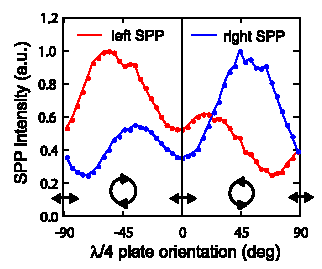
\includegraphics[width=\textwidth]{figures/RF_SM_Intensity.pdf}
			\caption{Intensitätsverteilung}
			\label{fig:RF_measure_int}
		\end{subfigure}
		\caption[Vergleichsmessung von \cite{RodriguezFortuno.2013}]{Die Abbildung zeigt die Messungen von \cite{RodriguezFortuno.2013}, die an einer Gitterstruktur durchgeführt worden sind.}			
	\end{figure}
	\newpage
	\section{Zusammenfassung und Ausblick}
	In dieser Arbeit wurde erfolgreich ein bestehendes Leckstrahlmikroskop modifiziert und in einigen Details verbessert.	Der Strahlgang des Lasers wurde so verändert, dass die Einkopplung des Lasers unter nicht senkrechtem Einfall auf die Probe erfolgen kann. Hierfür musste das Einkoppelobjektiv durch einen einfache Sammellinse ersetzt werden. Außerdem wurde ein Polfilter und eine $\lambda/4$-Platte zur Kontrolle der Polarisation des Lasers verbaut. Es wurden außerdem zahlreiche Optomechaniken modifiziert.
	
	Die Funktionsfähigkeit des LRM wurde durch zahlreiche Probemessung geprüft. Und abschließend konnte der plasmonische Spin-Hall-Effekt beobachtet werden. 
	
	
	\newpage
	\appendix
	\bibliography{bib}
	\section{Programmierung}
	\section{Weitere Messdaten}
	\begin{figure}[h!]
		\label{fig:dirt_measure}
		\centering
		\begin{subfigure}[b]{0.5\textwidth}
			\centering
			\includegraphics[width=\textwidth]{figures/dirt_radial.pdf}
			\caption{Radial-Profil}
			\label{fig:dirt_radial}
		\end{subfigure}
		\hfill
		\begin{subfigure}[b]{0.49\textwidth}
			\centering
			\includegraphics[width=\textwidth]{figures/dirt_lorentz.pdf}
			\caption{Lorentz-Fit}
			\label{fig:dirt_lorentz}
		\end{subfigure}
	
		\begin{subfigure}[b]{0.7\textwidth}
		\centering
		\includegraphics[width=\textwidth]{figures/dirt_polar.png}
		\caption{Intensitätsverteilung}
		\label{fig:dirt_polar}
		\end{subfigure}
		\caption[Messung an kontaminierter Probe]{Die Abbildung zeigt die BFP bei der Messung an einer mit Öl kontaminierten Probe unter senkrechtem Laser-Einfall. Der Wellenvektor wurde hier mit Hilfe eines Lorentz-Fits auf $k_\mathrm{SPP} = (11.0 + 0.4i)\,\mathrm{\mu m}^{-1}$ bestimmt. Die Dämpfung ist hier also signifikant größer als bei den Messungen an reinen Proben.}			
	\end{figure}

	\begin{figure}[h!]
		\label{fig:measure_polar}
		\centering
		\begin{subfigure}[b]{0.5\textwidth}
			\centering
			\includegraphics[width=\textwidth]{figures/spin_hall/polar/polar_45.png}
			\caption{$\alpha_{\lambda/4} = 45^\circ$}
			\label{fig:measure_polar_45}
		\end{subfigure}
		\hfill
		\begin{subfigure}[b]{0.49\textwidth}
			\centering
			\includegraphics[width=\textwidth]{figures/spin_hall/polar/polar_135.png}
			\caption{$\alpha_{\lambda/4} = 135^\circ$}
			\label{fig:measure_polar_135}
		\end{subfigure}
		
		\begin{subfigure}[b]{0.5\textwidth}
			\centering
			\includegraphics[width=\textwidth]{figures/spin_hall/polar/polar_0.png}
			\caption{$\alpha_{\lambda/4} = 0^\circ$}
			\label{fig:dirt_radia_0}
		\end{subfigure}
		\hfill
		\begin{subfigure}[b]{0.49\textwidth}
			\centering
			\includegraphics[width=\textwidth]{figures/spin_hall/polar/polar_90.png}
			\caption{$\alpha_{\lambda/4} = 90^\circ$}
			\label{fig:dirt_radia_90}
		\end{subfigure}
		\caption[BFP in Abhängigkeit der Abstrahlrichtung]{Die Abbildung zeigt die BFP bei der Messung an einem Punktdefekt unter streifenden Laser-Einfall.}			
	\end{figure}
		
	\section{Polarimeter}
	\newpage
	\section{Technische Zeichnungen}
	\begin{figure}[h!]
		\centering
		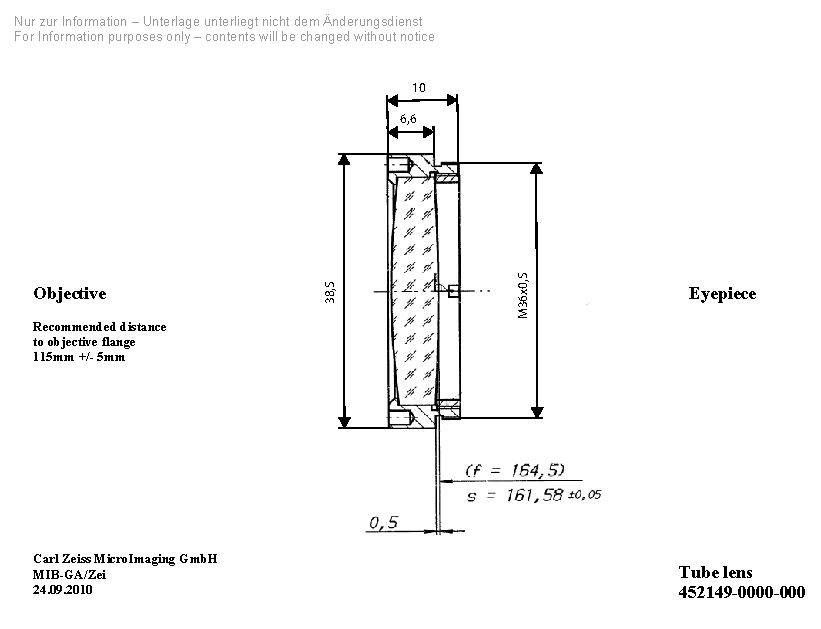
\includegraphics[width=1\linewidth]{figures/tube_lense_tz}
		\caption{Technische Zeichnung der Tubus-Linse}
		\label{fig:tubelensetz}
	\end{figure}
	
	\begin{sidewaysfigure}[h!]
		\includegraphics[width=\textwidth]{figures/Technische_Zeichnung_Probenhalter.pdf}
		\caption{Technische Zeichnung Probenhalter}
		\label{fig:tz_probenhalter}
	\end{sidewaysfigure}
	\begin{sidewaysfigure}[h!]
		\includegraphics[width=\textwidth]{figures/Probenblech.pdf}
		\caption{Technische Zeichnung Probenblech}
		\label{fig:tz_probenblech}
	\end{sidewaysfigure}
	\begin{sidewaysfigure}[h!]
		\includegraphics[width=\textwidth]{figures/LinsenAdapter.pdf}
		\caption{Technische Zeichnung Linsen-Adapter}
		\label{fig:tz_adapter}
	\end{sidewaysfigure}
	\begin{sidewaysfigure}[h!]
		\includegraphics[width=\textwidth]{figures/4f_system.pdf}
		\caption{Technische Zeichnung Cage-System}
		\label{fig:tz_cage_system}
	\end{sidewaysfigure}
	\newpage
	\section{Liste der verwendeten Komponenten}
	\begin{table}[h!]
		\centering	
		\begin{tabular}{|c|c|c|}
			\hline
			\textbf{Bauteil}         & \textbf{Typ}                   & \textbf{Hersteller}                    \\
			\hline
			\hline
			Helium-Neon-Laser        & HNL210L-EC                     & \textit{Thorlabs}                      \\
			ND Filter                & NDL-25C-2                      & \textit{Thorlabs}                      \\
			$\lambda/4$-Plättchen    & WPMQ05M-633                    & \textit{Thorlabs}                      \\
			Polarisationsfilter      & -        					  & \textit{Newport}                       \\
			Hintergrund LED          & -          					  & -                  					   \\
			Blenden                  & -          					  & -                  					   \\
			Spiegel                  & -          					  & -                  					   \\
			Kollimatorlinse          & Lens Asphere Ach 25x40Vis 0 TS & \textit{Edmund Optics}                 \\
			Immersionsobjektiv       & 100-fach/1.25 N-Achroplan      & \textit{Carl Zeiss}                    \\
			Immersionsöl             & 518N, n=1.518                  & \textit{Carl Zeiss}                    \\
			Tubuslinse               & 452149-0000-000                & \textit{Carl Zeiss}                    \\
			2x Linsen                & LA1417-A-ML, f = 150 mm        & \textit{Thorlabs}                      \\
			1x Linsen                & LA1417-A-ML, f = 75 mm         & \textit{Thorlabs}                      \\
			2x Lineartisch           & 2000551						  &\textit{Thorlabs} 					   \\
			Kristallhalter           & LP-1A (XYZ) Series             & \textit{Newport}                       \\
			Objektiv-Adapter         & LPMH-1                         & \textit{Newport}                       \\
			3-Achsen-Bühne           & TSD                            & \textit{OptoSigma}                     \\
			2-Achsen-Bühne           & TSD                            & \textit{OptoSigma}                     \\
			Filter-Halter            & FH2                            & \textit{Thorlabs}                      \\
			Einkoppellinse           & LA-1805                        & \textit{Thorlabs}                      \\
			Linsenhalter             & M-LH-1A                        & \textit{Newport}                       \\
			Cage Plate               & LCP08/M                        & \textit{Thorlabs}                      \\
			Linsen Tubus Verbinder   & CMT2                           & \textit{Thorlabs}                      \\
			SM2, CMount Adapter      & SM2A54                         & \textit{Thorlabs}                      \\
			Justierbarer Linsentubus & SM2V05                         & \textit{Thorlabs}                      \\
			Magnet Cage-Plate        & LCP90F                         & \textit{Thorlabs}                      \\
			3x xy-Linsenhalter       & CXY2                           & \textit{Thorlabs}                      \\
			3x Cage-System-Halter    & LCP01B                         & \textit{Thorlabs}                      \\
			4x Cage-System-Stange    & ER8                            & \textit{Thorlabs}                      \\
			4x Cage-System-Stange    & ER24                           & \textit{Thorlabs}                      \\
			4x Stangenverbinder      & ERSCB                          & \textit{Thorlabs}                      \\
			CageSystem Justier Hilfe & LCPA1                          & \textit{Thorlabs}                      \\
			CMOS IP-Kamera 			 & Mako G307C					  &	\textit{Allied Vision}				   \\
			Probenhalter		     & Eigendesign                    & Werkstatt                              \\
			Probenblech              & Eigendesign                    & Werkstatt                              \\
			BeamBlock                & Eigendesign                    & Werkstatt                              \\
			Tubuslinsenhalter        & Eigendesign                    & Werkstatt                              \\
			\hline          
		\end{tabular}
		\caption{Liste der verwendeten Komponenten}
		\label{tab:components}
	\end{table}
	
	
\end{document}
